
\documentclass[twocolumn]{article}
\usepackage{mathpazo}
\usepackage{microtype}
\usepackage{times}
\usepackage{titlesec} % 1
\usepackage[colorlinks = true,
            linkcolor = blue,
            urlcolor  = blue,
            citecolor = blue,
            anchorcolor = blue]{hyperref}
%\usepackage{sectsty} % "제 1 절" ...

 %%%%%%%%%%%%%%%%%%%%%%%%%%%%%%%%%%%%%%%%%%%%%%%%%%%%%%%%%%%%%%%%%%%%%%%%%%%%%
 %                              My Commands
\newcommand{\bi}{\begin{itemize}}
\newcommand{\ei}{\end{itemize}}
\newcommand{\be}{\begin{enumerate}}
\newcommand{\ee}{\end{enumerate}}
\newcommand{\ii}{\item}
\newtheorem{Def}{Definition}
\newtheorem{Lem}{Lemma}
\usepackage{algorithm}
\usepackage{algorithmicx}
\usepackage{algpseudocode}

\usepackage{graphicx}
\graphicspath{%
        {converted_graphics/}
        {./images/}
}

\usepackage{color}
\usepackage{xcolor}
\usepackage{listings}
\usepackage{caption}
\DeclareCaptionFont{white}{\color{white}}
\DeclareCaptionFormat{listing}{\colorbox{gray}{\parbox{\textwidth}{#1#2#3}}}
\captionsetup[lstlisting]{format=listing,labelfont=white,textfont=white}
\usepackage{verbatimbox}

\usepackage[hangul,nonfrench,finemath]{kotex}
    
\setlength\textwidth{7in} 
\setlength\textheight{9.5in} 
\setlength\oddsidemargin{-0.25in} 
\setlength\topmargin{-0.25in} 
\setlength\headheight{0in} 
\setlength\headsep{0in} 
%\setlength\columnsep{5pt}
\sloppy 
 
\begin{document}

\title{
\vspace{-0.5in}\rule{\textwidth}{2pt}
\begin{tabular}{ll}\begin{minipage}{4.75in}\vspace{6px}
\noindent\large {\it KIWI Project}@Data Management Research Section\\
\vspace{-12px}\\
\noindent\LARGE ETRI\qquad  \large Technical Report 15ZS1410-TR-65
\end{minipage}&\begin{minipage}{2in}\vspace{6px}\small
218 Gajeong-ro, Yuseong-gu\\
Daejeon, 305-700, South Korea\\
http:/$\!$/www.etri.re.kr/\\
http:/$\!$/sungsoo.github.com/\quad 
\end{minipage}\end{tabular}
\rule{\textwidth}{2pt}\vspace{0.25in}
\LARGE \bf GPU 가속 데이터 관리 기술에 관한 조사 \\
\large A Survey on GPU-Accelerated Data Management Technologies
}

\date{}

\author{
{\bf Sung-Soo Kim}\\
\it{sungsoo@etri.re.kr}
}

\maketitle

\begin{abstract}
GPU 상의 범용계산 접근법 (GPGPU)은 일반적으로 컴퓨터 그래픽스를 위한 계산만 맡았던 그래픽 처리 장치(GPU)를, 전통적으로 CPU가 맡았던 응용 프로그램들의 계산에 사용하는 기술이다. 
기존 CPU 클러스터 기반의 하둡을 GPGPU를 적용하여 더 빠른 처리성능을 얻을 수 있을까? 
이론적으로 처리해야 할 프로세스가 병렬 컴퓨팅에 최적화되어 있는 경우 GPU는 CPU보다 50배에서 100배까지 빠르게 연산을 수행한다.
하지만, GPGPU에서 주요 병목현상은 GPU 메모리와 CPU 메모리 사이의 PCIe 버스를 통한 느린 데이터 전송에서 발생한다. 
그래서 하둡과 같은 대규모 데이터 처리에 단순히 GPGPU의 처리방식만 적용하면 성능개선을 기대하기 어렵다.
현재까지 GPGPU기반 데이터관리 사례로는 하버드와 MIT에서 개발한 대규모 스트림데이터 처리/분석/가시화를 수행할 수 있는 시스템인 MapD \cite{mapd:2015}가 있지만, 대부분 GPGPU기반 하둡 연구들은 실험결과 제시수준이다.
GPGPU를 통해 하둡기반 빅 데이터 시스템의 성능을 높이기 위해서는 GPU상에서 다루어야 할 \textit{데이터 저장/압축모델}, \textit{처리 방식} 뿐만 아니라, \textit{질의 처리} 방식도 GPU에 최적화되어야 한다. 

KIWI 플랫폼의 질의 처리에 필요한 내부 성능 개선을 위해 GPGPU 접근법을 고려하고 있다. 
이와 관련하여 본 기술문서에서는 GPU 구조, 병렬화 특성, 최근 제안된 GPU기반 데이터 관리 기술들을 분석한다.
\end{abstract}

\section{Introduction}
In this section, we provide a brief overview of both a baseline GPU architecture, based primarily on NVIDIA’s G80/Fermi architecture, and GPGPU programming using the CUDA programming model.
\begin{figure}[htb]
        \centering
        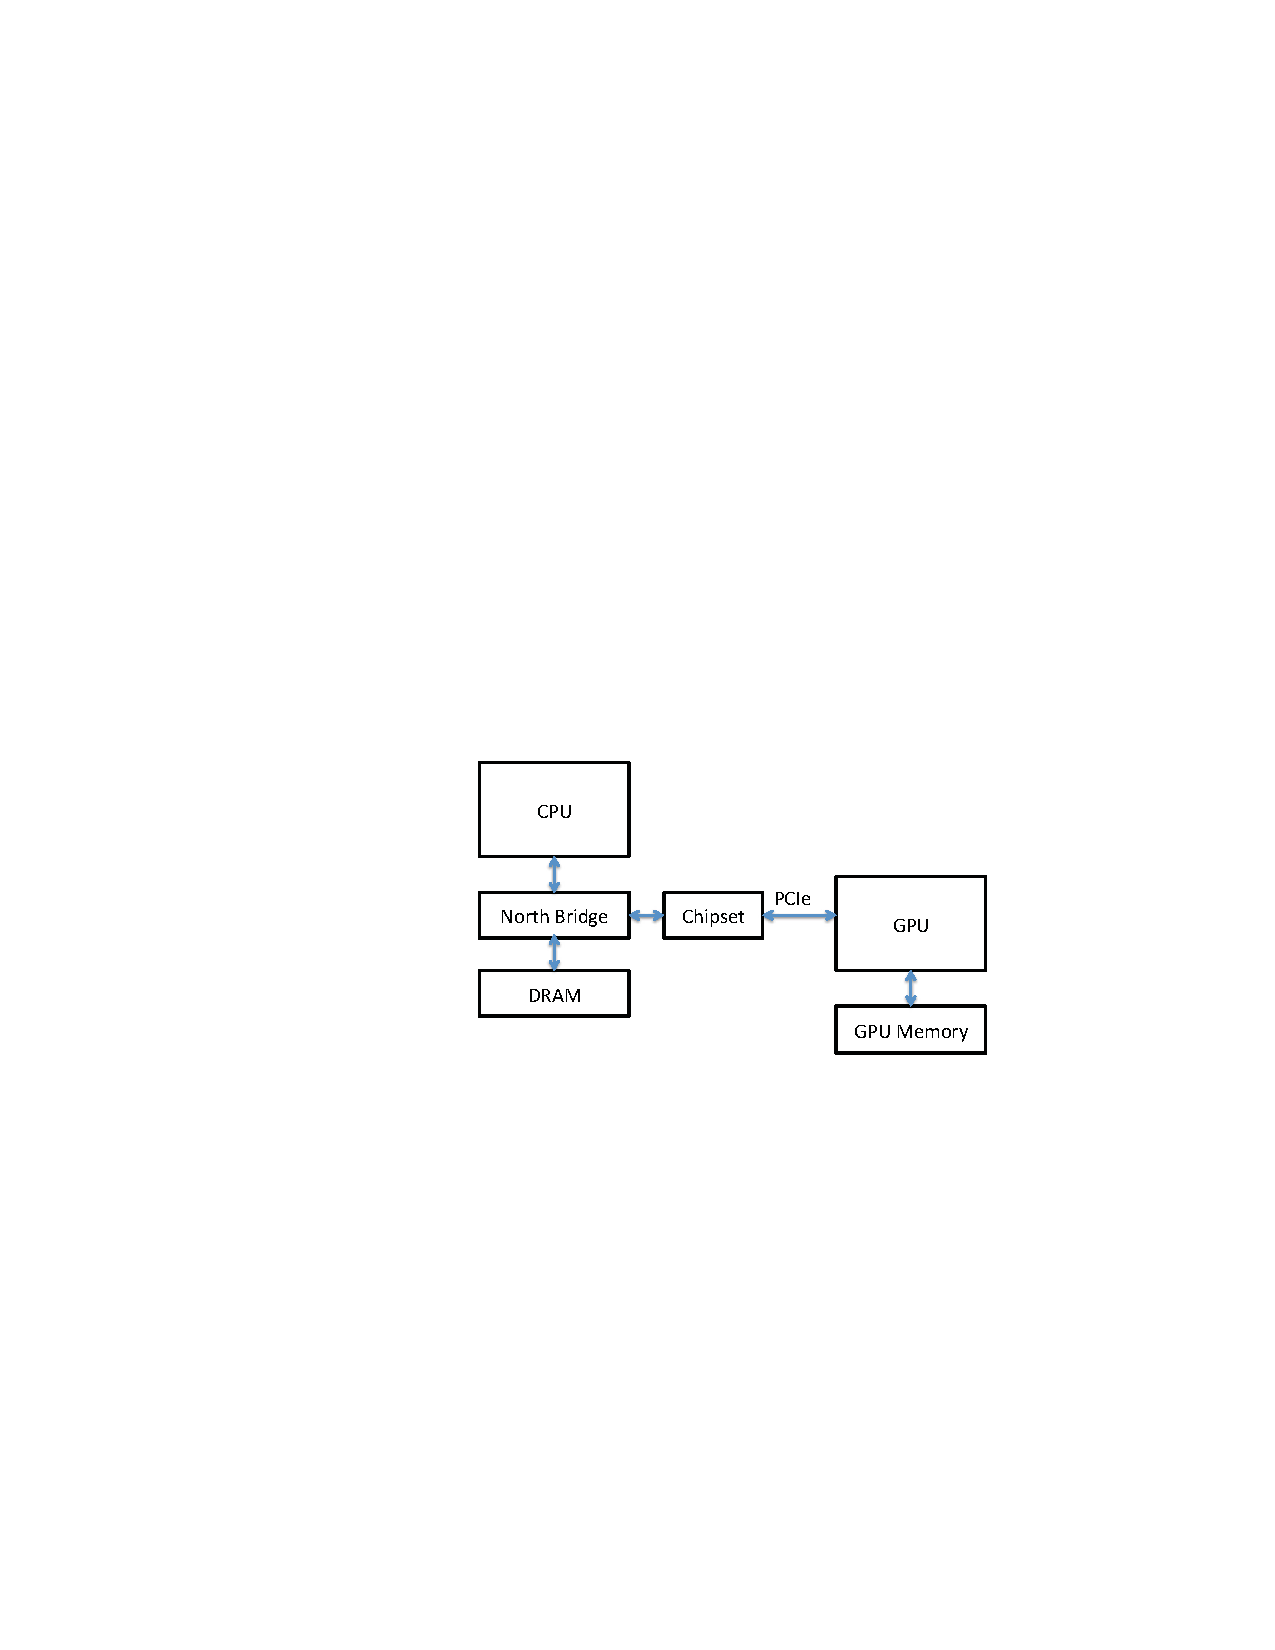
\includegraphics[width=0.48\textwidth]{system-overview.pdf}
        \caption{A system overview with CPU and a discrete GPU.}
        \label{fig:system_overview}
\end{figure}

Figure \ref{fig:system_overview} shows how a GPU is typically connected with a modern processor \cite{Kim:2012}. A GPU is an accelerator (or a co-processor) that is connected to a host processor (typically a conventional general-purpose CPU processor). The host processor and GPU communicate to each other via PCI Express (PCIe) that provides 4 Gbit/s (Gen 2) or 8 Gbit/s (Gen 3) interconnection bandwidth. This communication bandwidth often becomes one of the biggest bottlenecks; thus, it is critical to offload the work to GPUs only if the benefits of using GPUs outweigh the offload cost. The communication bandwidth is expected to grow as the CPU bus bandwidth of the system memory increases in the future.

\subsection{An Overview of GPU Architecture}
Figure \ref{fig:nvidia-g80} illustrates the major components of a general-purpose graphics processor, based on a simplified diagram of G80. At a high level, the GPU architecture consists of several streaming multiprocessors (SMs), which are connected to the GPU’s DRAM. (NVIDIA calls an SM and AMD calls a Compute Unit (CU).) Each SM has a number of single-instruction multiple data (SIMD) units, also called stream processors (SPs), and supports a multithreading execution mechanism. GPU architectures employ two important execution paradigms, which we explain below.
\begin{figure}[htb]
        \centering
        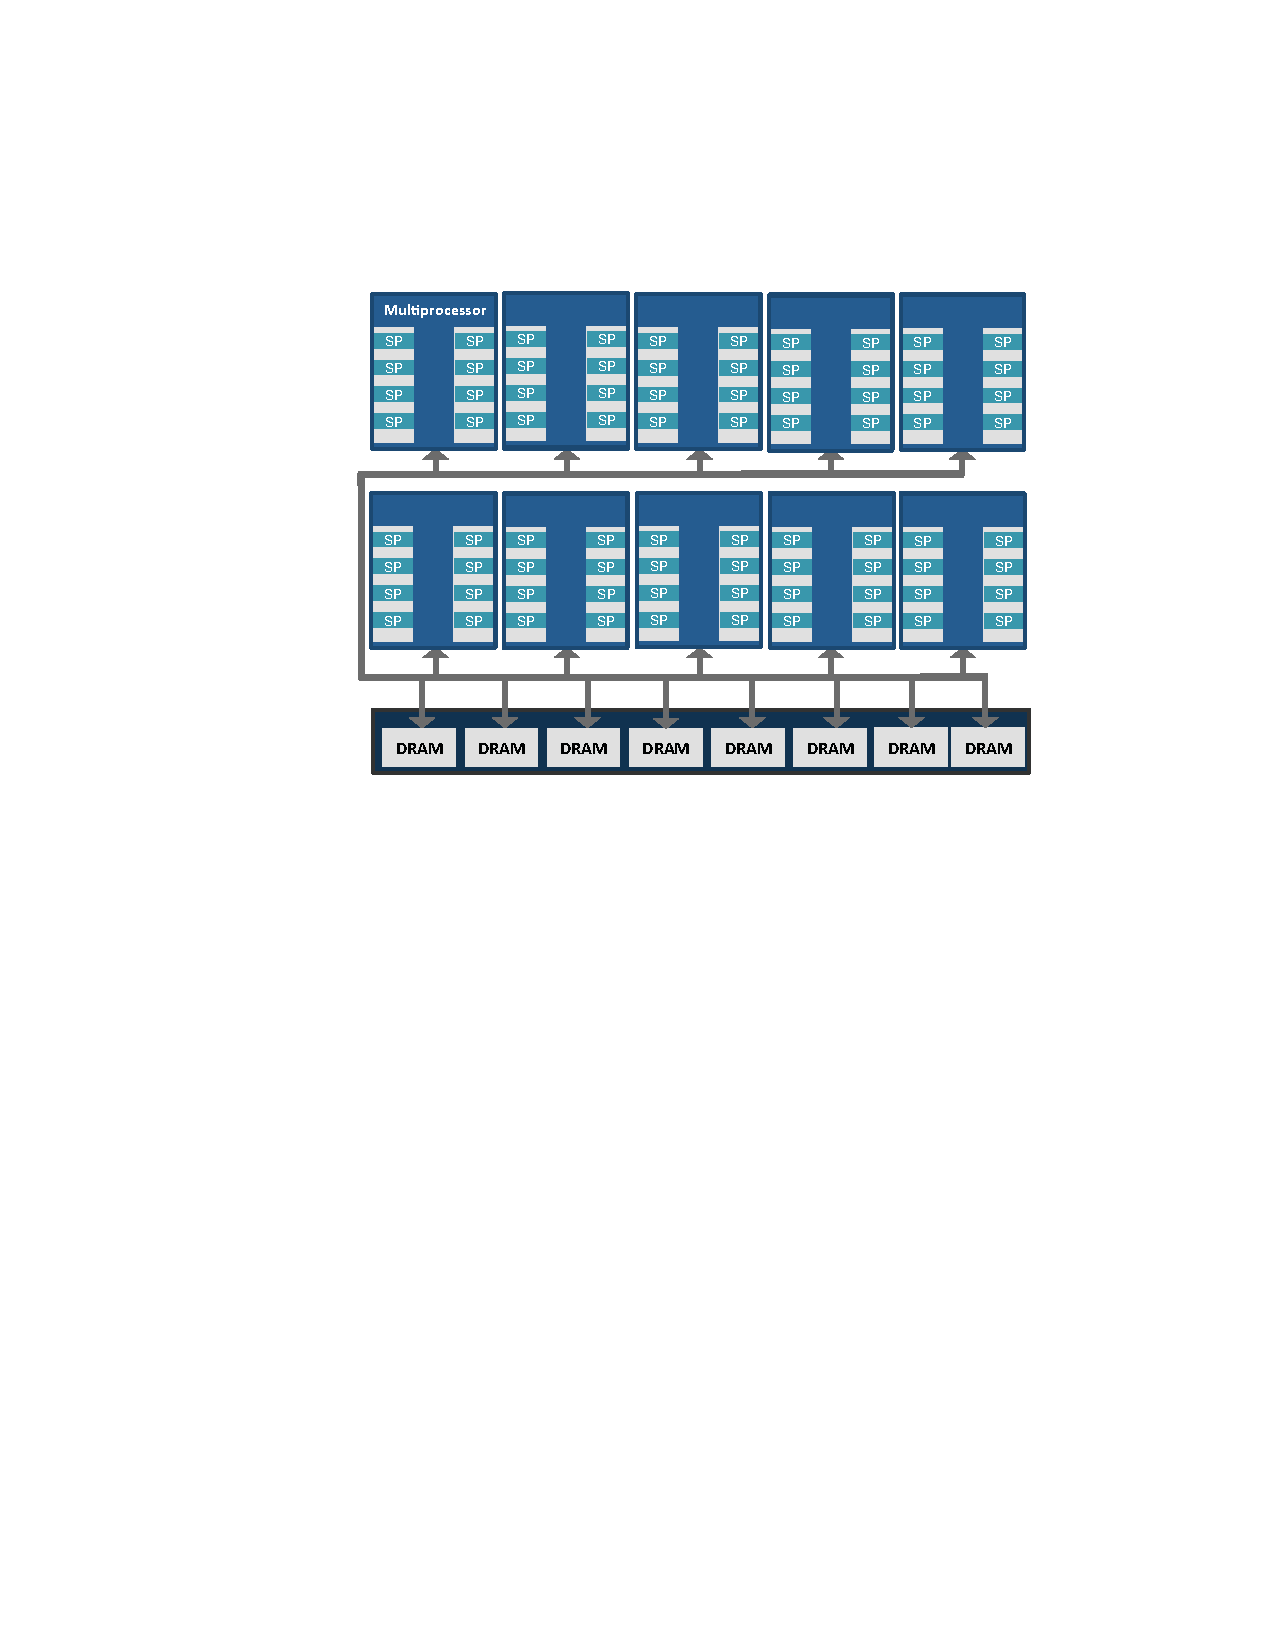
\includegraphics[width=0.48\textwidth]{nvidia-g80.pdf}
        \caption{Block diagram of NVIDIA’s G80 graphics processor (the components required for graphics processing are not shown).}
        \label{fig:nvidia-g80}
\end{figure}

\noindent
\textbf{SIMD/SIMT} 
GPU processors supply high floating-point (FP) execution bandwidth, which is the driving force for designing graphics applications. To make efficient use of the high number of FP units, GPU architectures employ a \textit{SIMD} or \textit{SIMT} execution paradigm. In SIMD, \textit{one instruction} operates on \textit{multiple data} (i.e., only one instruction is fetched, decoded, and scheduled but on multiple data operands). Depending on the word width, anywhere from 32, 64, or 128 FP operations may be performed by a single instruction on current systems. This technique significantly increases system throughput and also improves its energy-efficiency. This SIMD-style execution is essentially the same technique used in early vector processors. To support SIMD/vector operations, the register file should provide high bandwidth of read and write operations.

At a high level, the GPU programming model is based on the \textit{Single Program Multiple Data} (SPMD) model; a kernel function defines the program that is executed by each of the thousands of fine-grained threads that compose a GPU application. 

Since the programming model is SPMD, most of the threads perform the same work. Hence, a group of threads are executed in a lock-step fashion, executing the same instruction (on different data). This microarchitectural grouping of threads, which can affect both control flow and memory access efficiency, introduces the concept of \textit{warp}—a group of threads that are executed together in a lock step.

The execution model of G80 is called \textit{SIMT} (single instruction multiple threads). SIMT is very similar to SIMD with slight differences. When programmers write code, they can treat each thread separately. The program model allows each individual thread to perform different work. In contrast, in SIMD, the vector width is determined by the ISA level and one single instruction must perform the fixed vector width data at the same time. 

\noindent
\textbf{Multithreading} The other important execution paradigm that GPU architectures employ is \textit{hardware multithreading}. As in more conventional highly multithreaded architectures, such as HEP, M-Machine, Tera MTA, GPU processors use fast hardware-based context switching to tolerate long memory and operation latencies.

The effectiveness of multithreading depends on whether an application can provide a high number of concurrent threads. Most graphics applications have this characteristics since they typically need to process many objects (e.g., pixels, vertices, polygons) simultaneously. Multithreading is the key to understanding the performance behavior of GPGPU applications. In conventional CPU systems, thread context switching is relatively much more expensive: all program states, such as PC (program counter), architectural registers, and stack information, need to be stored by the operating system in memory. However, in GPUs, the cost of thread switching is much lower due to native hardware support of such process. Although modern CPUs also implement hardware multithreading (e.g., Intel’s \textit{hyperthreading}), thus far the \textit{degree} of multithreading (the number of simultaneous hardware thread contexts) is much lower in CPUs than in GPUs (e.g., two hyperthreads vs. hundreds of GPU threads).

To support multithreading in hardware, a processor must maintain a large number of registers, PC registers, and memory operation buffers. Having a large register file is especially critical. For example, the G80 architecture has a 16 KB first-level software managed cache (shared memory) while having a 32 KB register file. This large register file reduces the cost of context switch between threads. This fact is a key distinction from conventional CPU architectures.

\subsection{Design of GPU Architecture}
This section sketches the design of current GPU architectures. Much of this discussion pertains to NVIDIA’s Tesla/Fermi architectures. However, our descriptions are not intended to correspond directly to any existing industrial product.

\subsubsection{GPU Pipeline}
Figure \ref{fig:streaming-processor} shows an overview of a GPU architecture pipeline. It shows one streaming multiprocessor, which is based on an in-order scheduler. Similar to traditional architectures, it has fetch, decode, scheduler, register read, execution, and write-back stages.
\begin{figure}[htb]
        \centering
        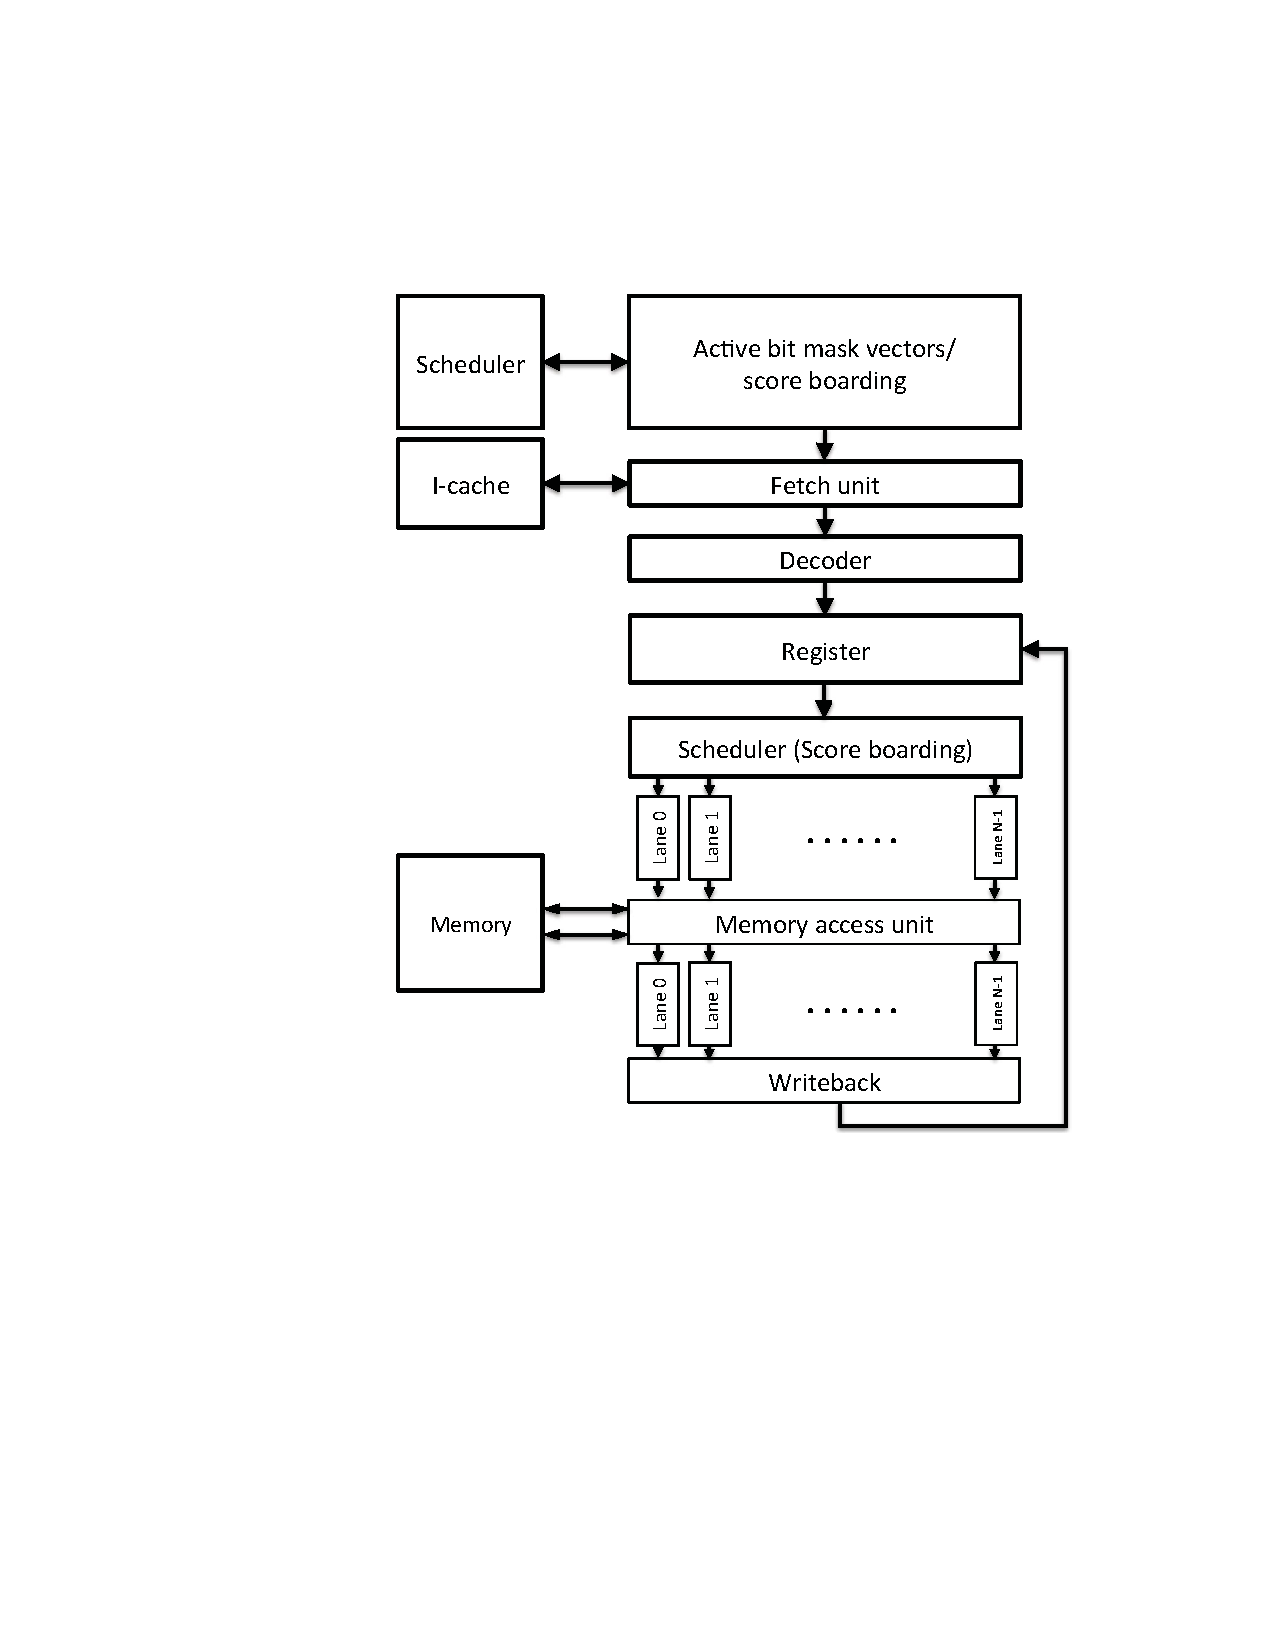
\includegraphics[width=0.48\textwidth]{gpu-streaming-pipeline.pdf}
        \caption{An overview of GPU streaming multiprocessor pipeline.}
        \label{fig:streaming-processor}
\end{figure}

\noindent
\textbf{Fetch and Decode Stage}
The front-end is very similar to traditional multithread architectures. Multiple PC registers exist to support multiple warps. The scheduler selects a warp to fetch based on scheduling algorithms, such as round-robin or greedy-fetch. The round-robin policy selects a warp from the list of ready warps, which gives an equal priority to each warp. In the greedy-fetch policy, the streaming multiprocessor fetches instructions from one warp until a certain event occurs such as I-cache miss or fetching a branch instruction or an instruction buffer full. Since the front-end has multiple warps to fetch, when it encounters such events, it simply switches to fetch another warp. For the same reason, branch predictors play a diminished role and are not typically implemented. Newer GPUs execute multiple warps at one cycle, so the front-end could fetch instructions from different warps at the same cycle instead of one warp at one cycle.

After an instruction is fetched, it is decoded in the decode stage. The streaming multiprocessor can have an instruction buffer for each warp or share a buffer for all warps.

\noindent
\textbf{Scheduler and Score Boarding} 
The GPU processor has an in-order scheduler. In the G80 architecture, it executes only one warp at a time; later architectures like Fermi schedule multiple warps. The scheduler uses a scoreboard to find a ready warp. So far, no GPU architectures have employed out-of-order schedulers. However, the scheduler can select any warps that are ready. Hence, from a programmer’s view point, a program might look like an out-of-order execution. For example, the scenario in Figure \ref{fig:intruction-traces} is possible.
\begin{figure}[htb]
        \centering
        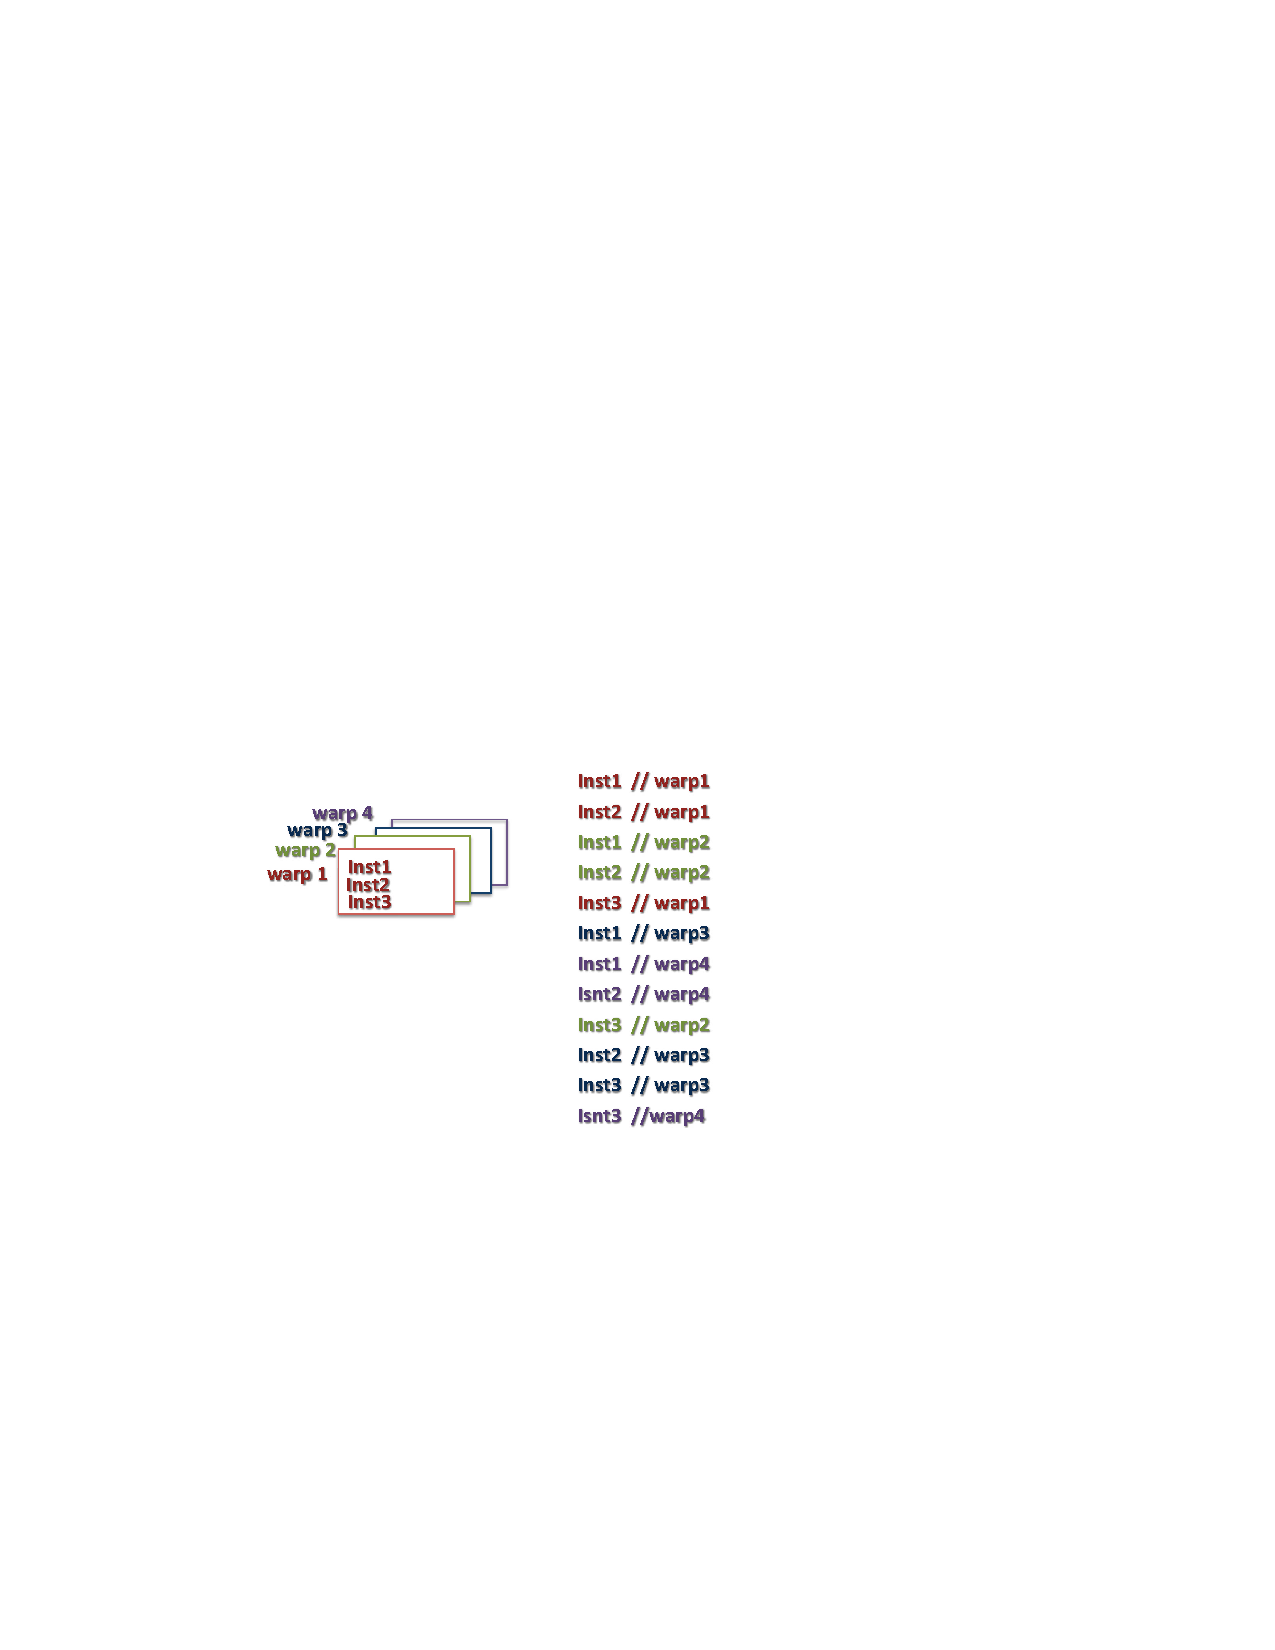
\includegraphics[width=0.48\textwidth]{instruction-traces.pdf}
        \caption{An example of static and dynamic instruction traces.}
        \label{fig:intruction-traces}
\end{figure}

\noindent
\textbf{Scoreboarding} \textit{Scoreboarding} is one method to implement dynamic scheduling. It was first introduced in CDC6600. It checks read-after-write and write-after-write data dependencies. Scoreboarding does not provide the register renaming mechanism, but instructions can execute out of order (i.e., instructions should be scheduled in-order but can be finished (complete functional units/memory accesses) out of order) when there are no conflicts and the hardware is available. In GPUs, scoreboarding is used to check any RAW or WAW dependency, so instructions from the same warp can be executed even if earlier instructions have not finished yet. This approach increases instruction/memory-level parallelism. 

\noindent
\textbf{Register read/write}
To accommodate a relatively large number of active threads, the GPU processor maintains a large number of register files. For example, if a processor supports 128 threads and each thread uses 64 registers, in total 128×64 registers are needed. As a result, the G80 has a 64 KB register file and the Fermi supports 128 KB of register file storage per streaming multiprocessors (in total, a 2 MB register file). The register file should have a high capacity and also high bandwidth. If a GPU has 1 Tflop/s peak performance and each FP operation needs at least two register reads and one register write, 2 T*32 B/s=64 TB/s register read bandwidth is required. Providing such high bandwidth is particularly challenging, so several techniques have been used, including multiple banks and operand buffer/collectors.
\begin{figure}[htb]
        \centering
        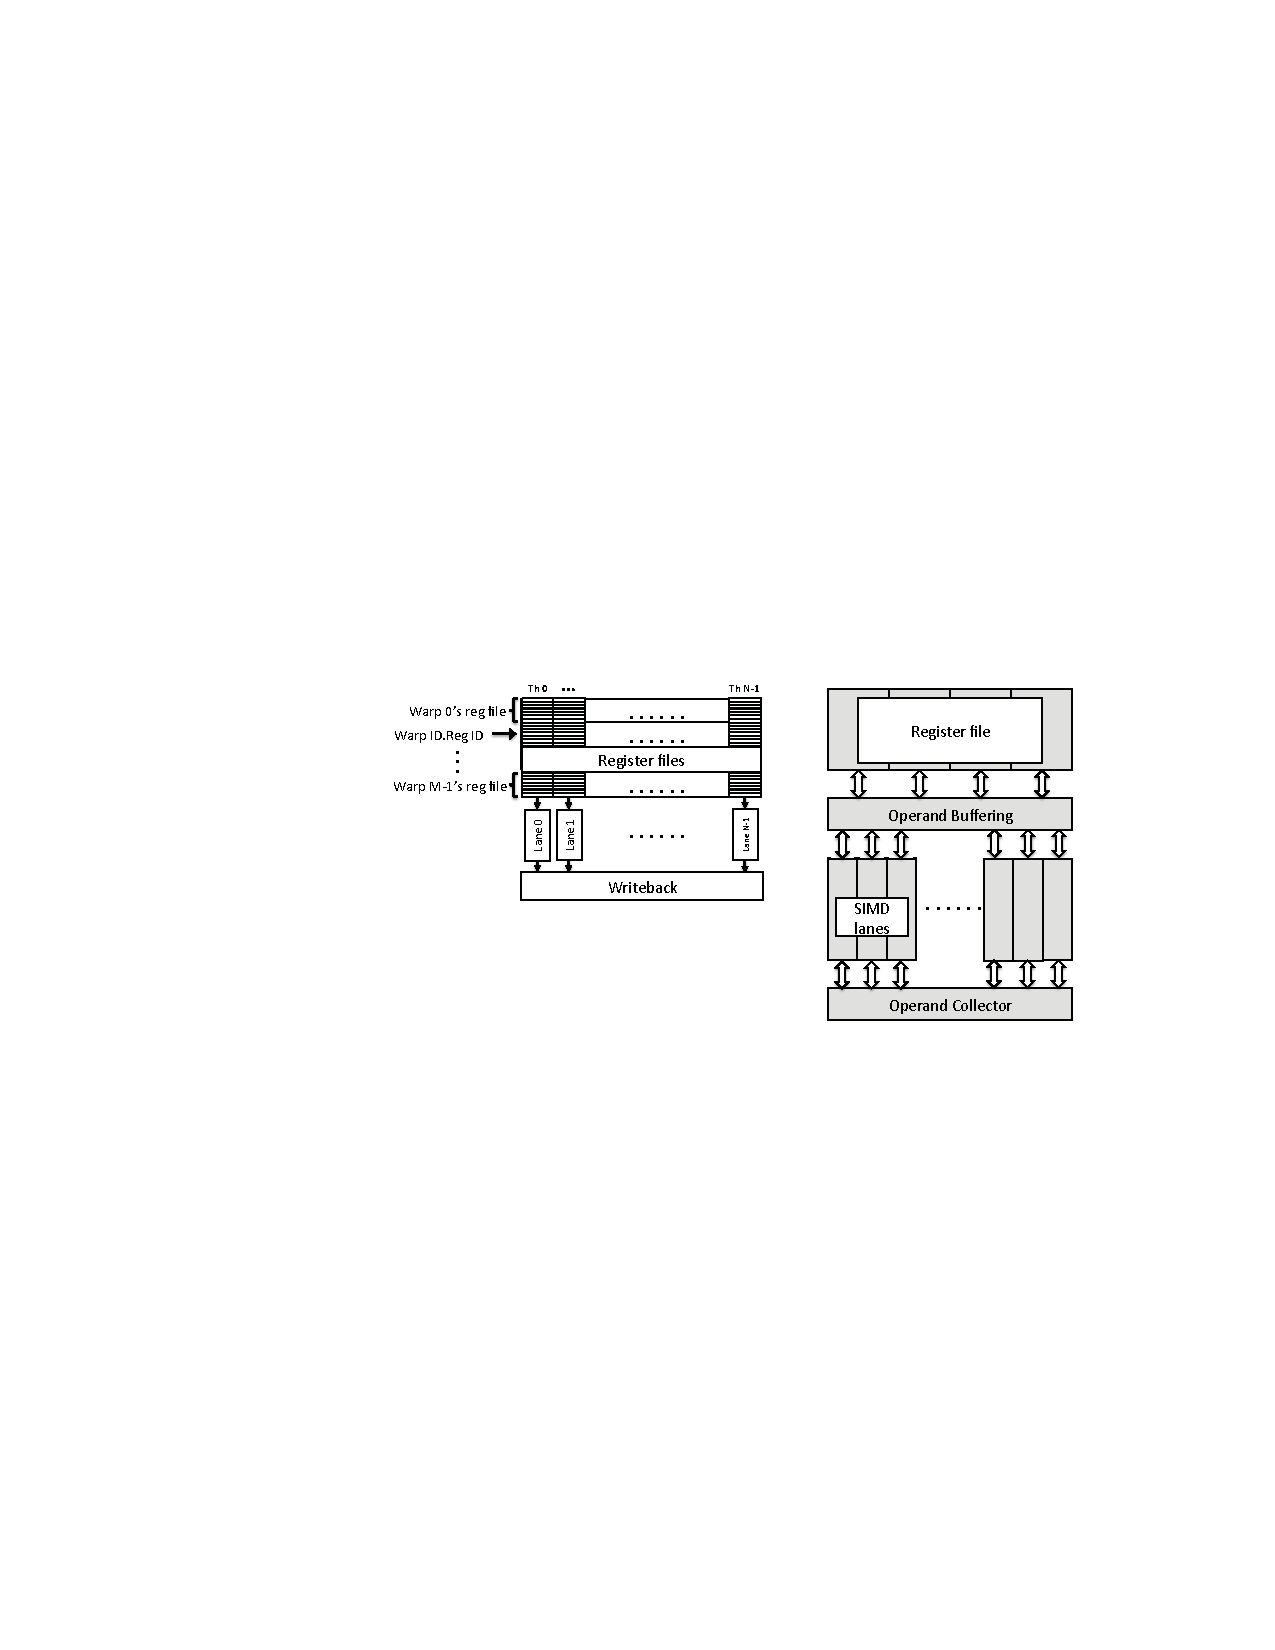
\includegraphics[width=0.48\textwidth]{register-file.pdf}
        \caption{GPU register file accesses. Left: using multiple banks; right: using operand buffering}
        \label{fig:register-file}
\end{figure}

\noindent
\textbf{Multiple banks} 
The streaming multiprocessor provides high bandwidth by subdividing the register file into multiple banks. 
Figure \ref{fig:operand} shows the register file structure. All threads in the warp read the register value in parallel from the register file indexed by both warp ID and register ID. Then, these register values are directly fed into the SIMD backend of the pipeline. (Please remember that each SIMD unit/lane is used by only one thread.)

\noindent
\textbf{Operand Buffer} 
Gebhart et al.  show another example of the register file structure in Figure \ref{fig:operand} . In that design, a buffer exists between the register file and the execution units. Instead of
reading all the necessary register values right before the values are needed, which gives a very high pressure to the register file read/write ports, the processor can buffer the register values.
The buffer can store register values that are read through multiple cycles, thereby reducing the register read bandwidth requirement. In their design, four SIMT lanes form a cluster. Each entry in the streaming multiprocessor’s main register file is 128 bits wide, with 32 bits allocated to the same-named register for threads in each of the four SIMT lanes in the cluster. Several documents indicate that they employ operand collector buffers. These operand collectors are also used to aggregate result values. The operand collector works as a result queue, which buffers the output from functional units before being written back into the register file. Although the main benefit of the result queues is to increase the effective write throughputs, it also provides further optimization opportunities. When the outcomes of instructions are used only in the instructions dynamically scheduled close enough, the output values can be forwarded to the input of the next operation. This behaves just like a CPU’s forwarding network.

When an instruction requires multiple accesses to the same bank, the register values are read over multiple cycles. Since the register addresses are determined statically, the compiler can in principle reduce or remove bank conflicts.
\begin{figure}[htb]
        \centering
        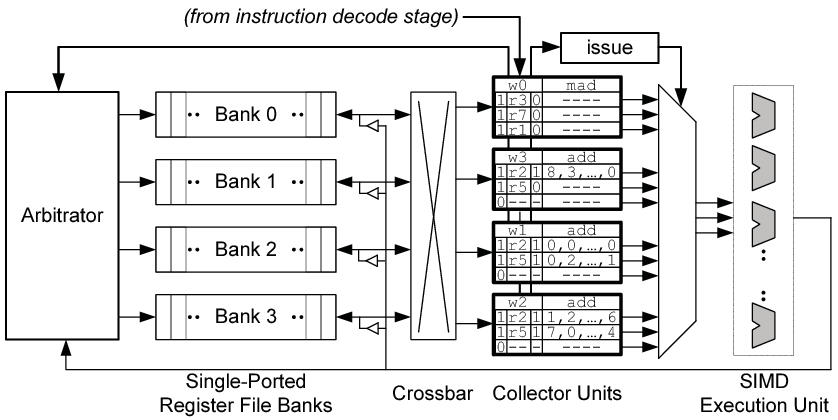
\includegraphics[width=0.48\textwidth]{operand.jpg}
        \caption{Detailed diagram of Operand Collector}
        \label{fig:operand}
\end{figure}

\noindent
\textbf{Register File Cache} 
To reduce the pressure on the register file, Gebhart et al. propose a \textit{register file cache}. Although a register file cache was originally proposed to reduce the register file access time, in GPUs the register file cache is proposed to reduce register reads and writes. Current GPU architectures do not support precise exceptions, so register files do not have to maintain architectural states. Therefore, many write operations can be easily merged inside the register file cache, which may reduce register writes significantly.

\noindent
\textbf{Execution stage}
In the execution stage, an instruction accesses either the memory unit or functional units. 
The execution stage consists of \textit{vector processing units} (AMD GPUs have a scalar unit as well). One vector lane executes one thread, which is called a stream processor in NVIDIA's terminology. The simplest design would be to have the number of lanes and the warp size be the same. However, this approach could also require a relatively large amount of static power consumption and a large area. Instead, GPUs execute the same instruction over multiple cycles. For example, the G80 has only 8 vector lanes, and therefore the streaming multiprocessor takes four cycles to execute 32 threads (i.e., one warp). The computed results are temporarily stored and then written back to the register file together.

\noindent
\textbf{Back-to-back operation} 
The execution width of GPU is wide (32 threads), which makes it much harder to have a data forwarding path. For example, 32 × 32 B (total 1 KB) or 32 × 64 B (total 2 KB) widths are quite large. Hence, the results are either written directly to the register file or temporarily stored in a small buffer and then written back to the register file over multiple cycles. In either case, the results are not available to dependent instructions immediately after execution. This scenario is quite different from many modern CPUs, where data forwarding is used widely. When there is a forwarding path, register read/write cycles are not in the critical path and any back-to-back operations are executed immediately following the execution latency. However, GPUs can avoid this penalty by utilizing \textit{thread-level parallelism} (TLP). The pipeline simply schedules instructions from other warps so it can hide the latency. When there is enough TLP, the execution and register write latency can be hidden.

Volkov discussed this issue in his GTC'10 talk. When there are four threads, the streaming multiprocessor can simply switch to other threads so the execution latency can be hidden. However, when there is only one thread, these back-to-back operations take much longer. 

\noindent
\textbf{Special function units} 
To date, NVIDIA architectures have adopted SIMD execution units and AMD architectures have used VLIW architectures. In addition, special function units provide VLIW-like effects in NVIDIA GPU architectures. Graphics applications often require transcen- dental functions for algorithms such as geometric rotations and scaling. It is often possible to use implementations of the corresponding transcendental functions that do not have ultra-high accuracy. Many GPU architectures therefore provide fast, approximate implementations in hardware-based special function units (SFUs). Since many programs do not need these SFUs all the time, the pro- cessor has only two-four SFUs in addition to its regular FP units. The scheduler can issue SFU instructions and regular FP instructions together if they are independent, e.g., when the instructions come from different warps. In such cases, these SFU units provide additional execution bandwidth. 

\subsection{Programming a GPU}
Programs that run on a graphics card are written in the so-called \textit{kernel programming model}. 
Programs in this model consist of \textit{host code} and \textit{kernels}. The host code manages the graphics card, initializing data transfer and scheduling program execution on the device. A kernel is a simplistic program that forms the basic unit of parallelism in the kernel programming model. Kernels are scheduled concurrently on several scalar processors in a SIMD fashion: Each kernel invocation - henceforth called \textit{thread} - executes the same code on its own share of the input. All threads that run on the same multiprocessor are logically grouped into a \textit{workgroup}.

One of the most important performance factors in GPU programming is to avoid data transfers between host and device: All data has to pass across the PCIexpress bus, which is the bottleneck of the architecture. Data transfer to the device might therefore consume all time savings from running a problem on the GPU. This becomes especially evident for I/O-bound algorithms: Since accessing the main memory is roughly two to three times faster than sending data across the PCIexpress bus, the CPU will usually have finished execution before the data has even arrived on the device.

Graphics cards achieve high performance through massive parallelism. This means, that a problem should be easy to parallelize to gain most from running on the GPU. Another performance pitfall in GPU programming is caused by divergent code paths. Since each multiprocessor only has a single instruction decoder, all scalar processors execute the same instruction at a time. If some threads in a workgroup diverge, for example due to data-dependent conditionals, the multiprocessor has to serialize the code paths, leading to performance losses. While this problem has been somewhat alleviated in the latest generation of graphics cards, it is still recommended to avoid complex control structures in kernels where possible.

Currently, two major frameworks are used for programming GPUs to accelerate database systems, namely the \textit{Compute Unified Device Architecture} (CUDA) and the \textit{Open Compute Language} (OpenCL). Both frameworks implement the kernel programming model and provide API’s that allow the host CPU to man- age computations on the GPU and data transfers between CPU and GPU. In contrast to CUDA, which supports NVIDIA GPUs only, OpenCL can run on a wide variety of devices from multiple vendors.
However, CUDA offers advanced features such as allocation of device memory inside a running kernel or \textit{Uniform Virtual Addressing} (UVA), a technique where CPUs and GPUs share the same virtual address space and the CUDA driver transfers data between CPU and GPU transparently to the application.

\section{Performance Principles}
Developing algorithms for GPGPUs is fundamentally about applying the same long-studied principles of parallelization and I/O-efficient design relevant to other shared memory parallel platforms. 
In this section, we reviews these principles, focusing on recent results in both the theory and practice of parallel algorithms, and suggests a connection to GPGPU platforms. Ideally, applying these principles with the right cost models leads not only to provably efficient algorithms, but also offers hints to architects about the features and configurations likely to have the most impact on the performance of a given computation. Thus, we believe this discussion will be useful to practitioners in various aspects of parallel computing, not just those interested specifically in GPGPUs.

\subsection{Algorithm Design Models Overview}
The two most important characteristics of any algorithm likely to determine its performance are: (a) how much parallelism is available and (b) how much data must move through the memory hierarchy. Thus, when designing an algorithm, we would like an abstract machine model that allows us to assess our algorithm along these dimensions. In such a model, we might want to do the same kind of “big-O” analysis to which we are accustomed in the sequential case. Doing so would allow us to get the high-level algorithm design right before moving on to lower-level performance optimization and tuning. Importantly, the abstractions should not be so cumbersome that we cannot in a reasonable amount of time design and analyze candidate algorithms.

Although the state of algorithm design models is in flux, we have reasonable options. For GPGPUs and other manycore-style processors, two suitable models are the so-called \textit{work-depth} (or \textit{work-span}) model for analyzing parallelism, and the external memory model for analyzing I/O behavior in the presence of a memory hierarchy. These two models evolved separately, but recent work has shown ways in which to connect them. 

\subsection{Characterizing Parallelism}
In the \textit{work-depth model}, we represent a computation by a \textit{directed acyclic graph} (DAG) of operations, where edges indicate dependencies, as illustrated in Figure \ref{fig:worker-depth}. 
Given the DAG, we measure its \textit{work}, $W(n)$, which is the total number of unit-cost operations for an input of size $n$, and its \textit{depth} or \textit{span}, $D(n)$, which is its critical path length measured again in unit-cost operations. 
Note that $D(n)$ ought to be a lower bound on the minimum execution time, and the ratio $W(n)/D(n)$ effectively measures the average amount of available parallelism as each critical path node executes. 
In fact, the ratio $D(n)/W(n)$ is similar to the concept of a sequential fraction, as one might use in evaluating Amdahl’s Law. 
Thus, our implicit goal is to maximize $W (n)/D(n)$, or, alter- natively, minimize $D(n)/W(n)$. 
Importantly, this model makes no explicit reference to the number of processors. 
In this sense, we may regard the model as being machine-independent. 
Nevertheless, if we want to know how many processors to throw at an algorithm, $W (n)/D(n)$ is a suitable guide.
\begin{figure}[htb]
        \centering
        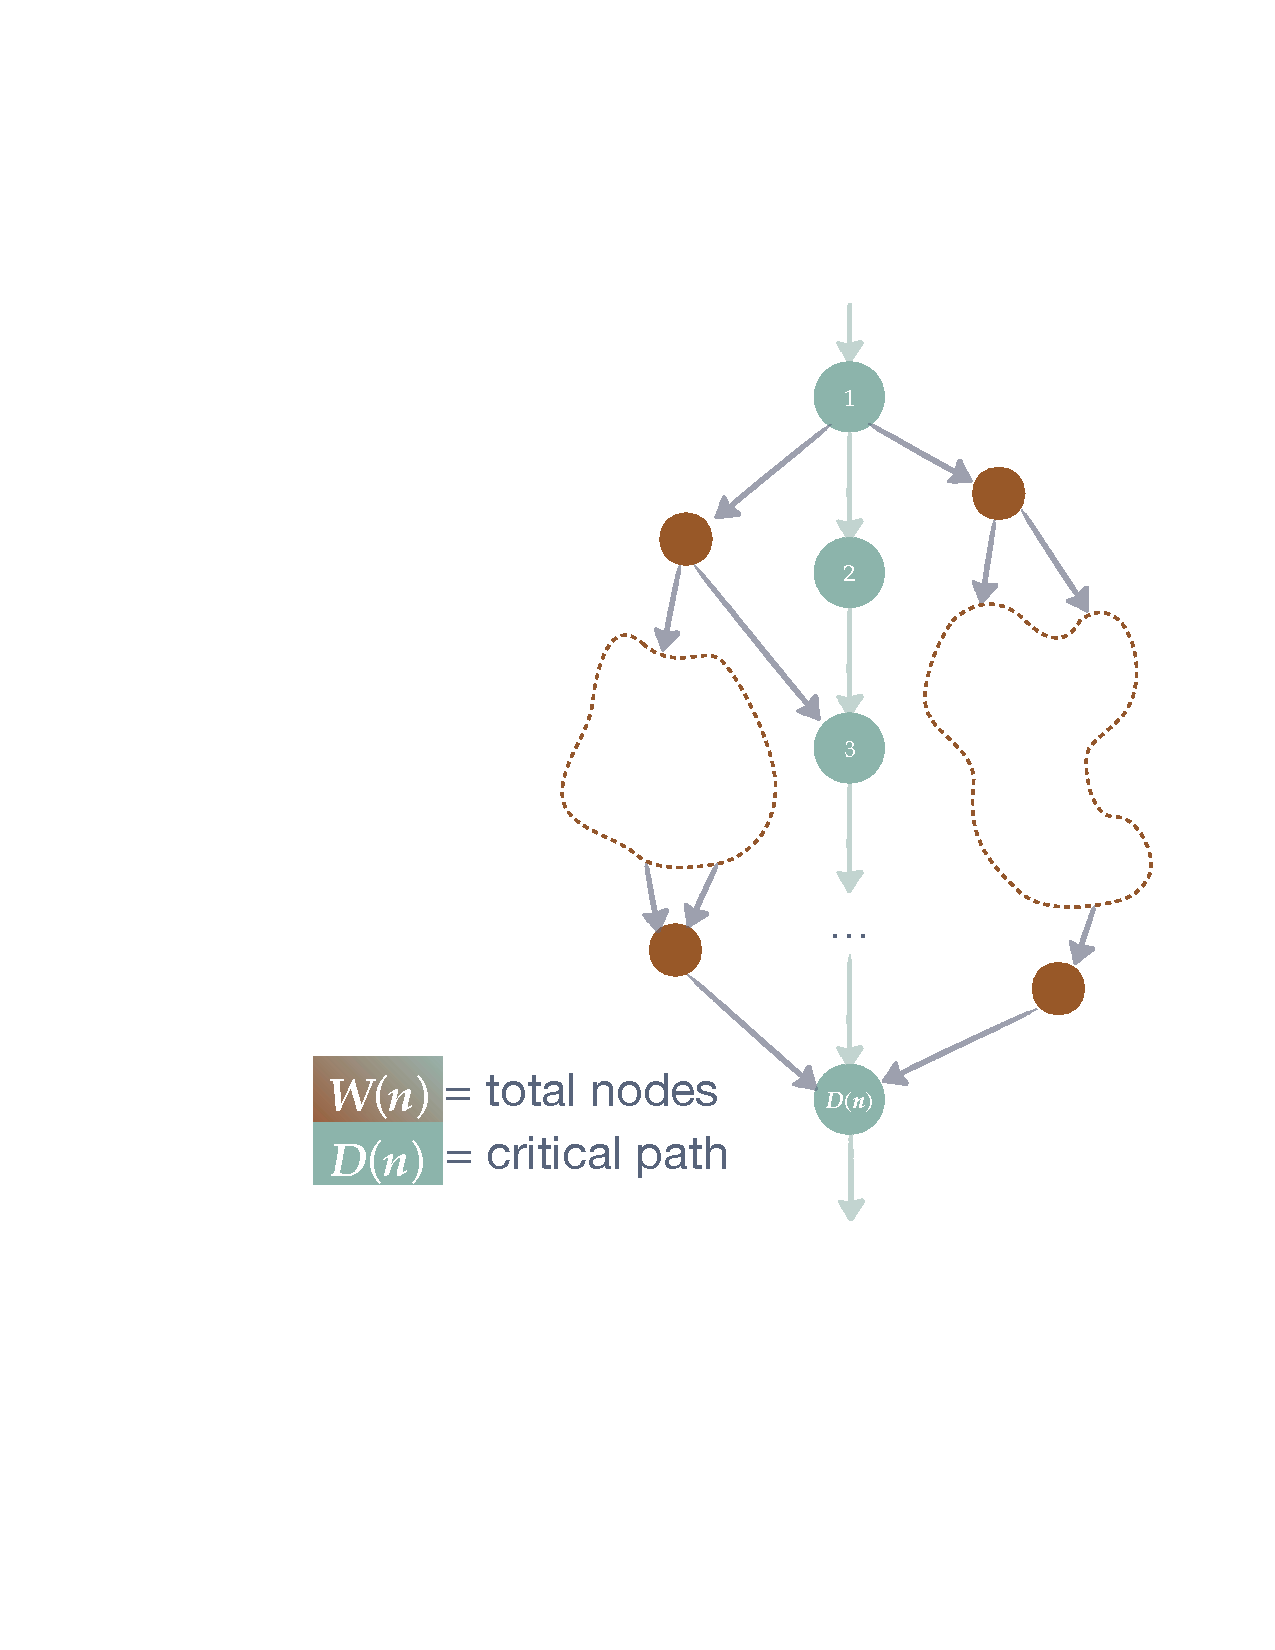
\includegraphics[width=0.38\textwidth]{work-depth-model.pdf}
        \caption{A parallel computation in the work-depth (or work-span) model. The computation for an input of size $n$ is a directed acyclic graph with $W(n)$ nodes, each representing a unit-cost operation; edges representing strict dependencies among these operations; and a critical path of length $D(n)$ nodes. Our goal is to design algorithms that achieve \textit{work-optimality} while maximizing the average available parallelism, $W (n)/D(n)$.}
        \label{fig:worker-depth}
\end{figure}

However, it is easy to maximize $W(n)/D(n)$ and still get a bad algorithm. 
For instance, we can artificially inflate the total operations $W (n)$. 
Thus, we should also try to ensure our algorithm is \textit{work-optimal}, a property which says that $W (n)$ is not asymptotically worse than the best sequential algorithm. Indeed, work-optimality is a critical requirement.

Let’s see why work-optimality matters. 
First, note that it is possible to estimate (crudely) the algorithm’s running time given $p$ identical processors, using a theorem by Brent. This theorem says that if the nodes of the DAG have unit cost and the machine has p processors, then it is possible to schedule the DAG so that the time to execute (compute) the DAG, $T_{comp}(n; p)$, is
\begin{equation}
T_{comp}(n; p) = D(n) + \frac{W(n) - D(n)}{p}
\label{eqn:cost}
\end{equation}
Suppose we have designed a highly parallel algorithm, with $W (n) \gg p \cdot D(n)$, and furthermore that our algorithm only exceeds the work $W_0(n)$ of the best sequential algorithm by a factor of $\varepsilon(n)$, i.e., $W(n) = W0(n) \cdot \varepsilon(n)$. 
Then, the speedup of our algorithm on p processors is roughly $W0(n)/(W(n)/p)=p/\varepsilon(n)$.
That is, the best possible speedup of p will be reduced by $\varepsilon(n)$.
Consider the relatively small factor of $\varepsilon(n) = \log n$. Even for $n = 1024$, $\log n = 10$, meaning the best possible speedup is an order of magnitude less than we might hope for. 
Put another way, to even match the sequential algorithm, we need $p >\varepsilon(n)$. 
Thus, if we are deciding between an $O(n)$ sequential algorithm and an $O(n^2/p)$ parallel algorithm, we will need $p = n$ just to match the sequential case. These examples underscore the importance of work-optimal algorithms.

\noindent
\textit{\textbf{Example: Reduction.}} 
Suppose we wish to compute the sum of n values. A sequential algorithm would lead to a DAG like the one shown in Figure \ref{fig:worker-depth-example}. 
In this case, we perform $\Theta(n)$ operations but the critical path is also of length $\Theta(n)$. 
Thus, the available parallelism—-or ratio of $W (n)/D(n)$—-is a constant: no matter how large the input, there is never more than a fixed amount of concurrency.
\begin{figure}[htb]
        \centering
        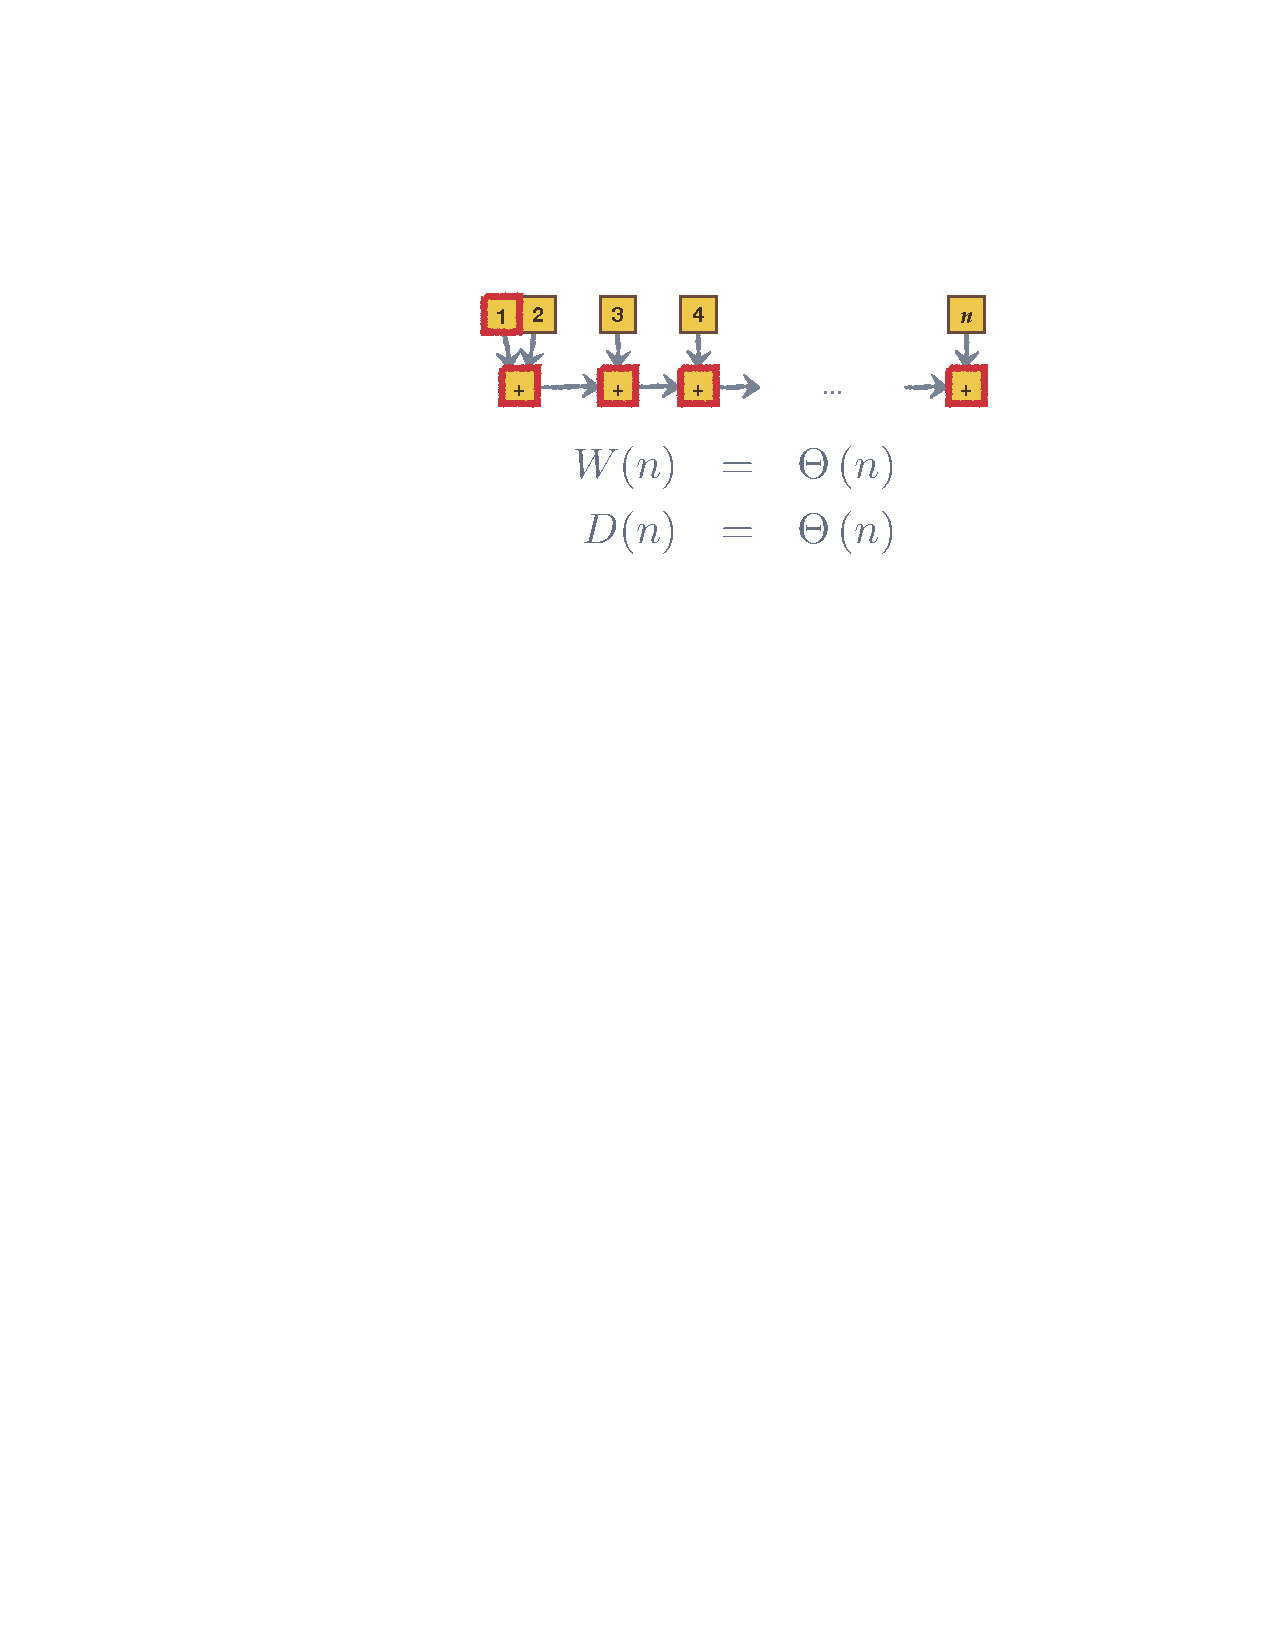
\includegraphics[width=0.35\textwidth]{work-depth-example.pdf}
        \caption{Work-depth example: summing a list of $n$ elements with a sequential algorithm. Both the work and the depth are $\Theta(n)$, meaning the available parallelism $W (n)/D(n)$ is a constant.}
        \label{fig:worker-depth-example}
\end{figure}

An algorithm with more parallelism might instead have the DAG shown in Figure \ref{fig:worker-depth-16}. 
\begin{figure}[htb]
        \centering
        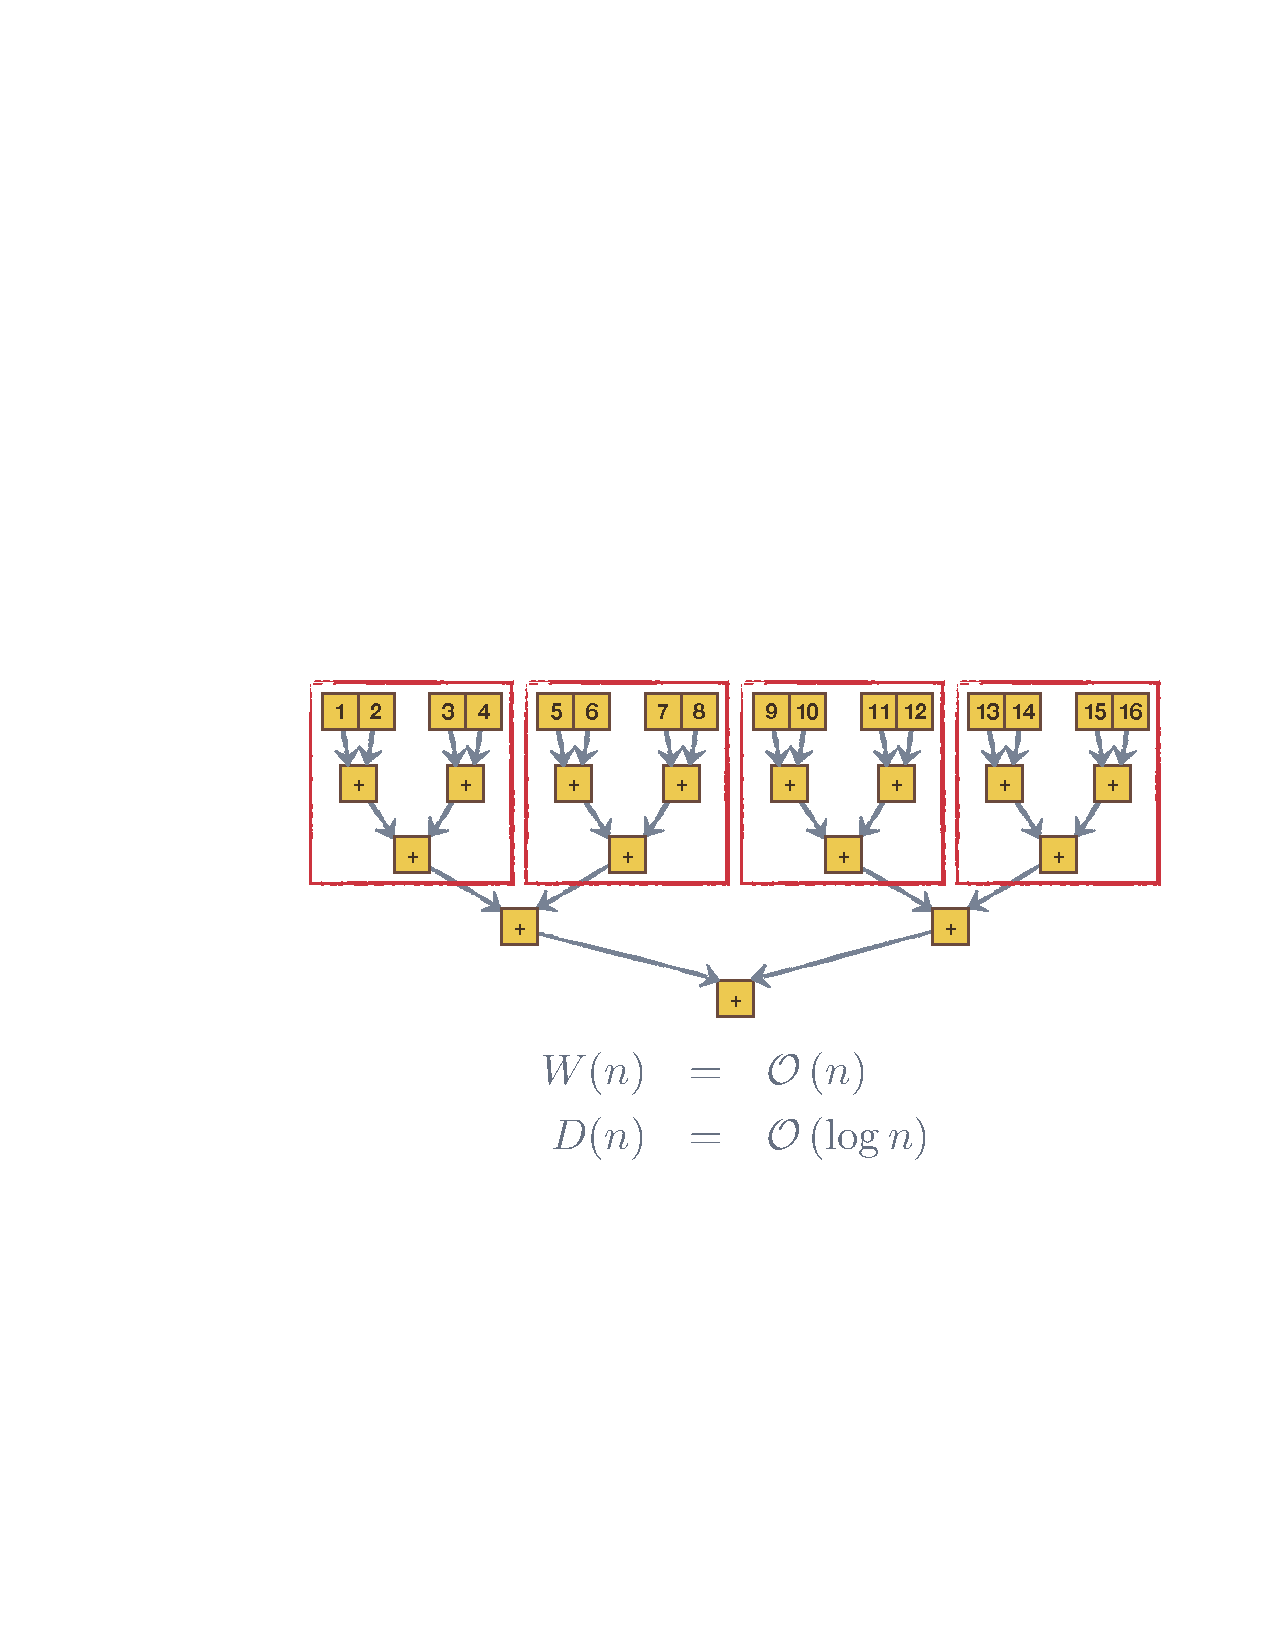
\includegraphics[width=0.49\textwidth]{work-depth-16.pdf}
        \caption{Work-depth example: summing a list of $n = 16$ elements with a tree algorithm.}
        \label{fig:worker-depth-16}
\end{figure}
This algorithm organizes the additions into a tree, where independent subtrees can be performed in parallel. 
This tree still performs $W (n) =\Theta(n)$ total operations, and is thus work-optimal. 
However, the depth of this DAG is just $D(n) =\Theta(\log n)$, the height of the tree. 
Thus, as $n$ grows, so does the average available parallelism, in the amount of $W (n)/D(n) =\Theta(n/ \log n)$. 
By this measure, this algorithm is a better one than the sequential algorithm, just as we would expect.
In the specific case of Figure \ref{fig:worker-depth-16}, where $n = 16$, the work $W (16) = 31$ nodes and the depth $D(16) = 5$. (Imagine that the “input” nodes at the top of Figure \ref{fig:worker-depth-16} represent load operations to retrieve the values.) Then, $W (16)/D(16) = 31/5 = 6.2$. Thus, there are an average of  $\approx 6$ nodes available to be executed in parallel during the computation. This implies that we could not gainfully use more than about six “processors.”
\begin{figure}[htb]
        \centering
        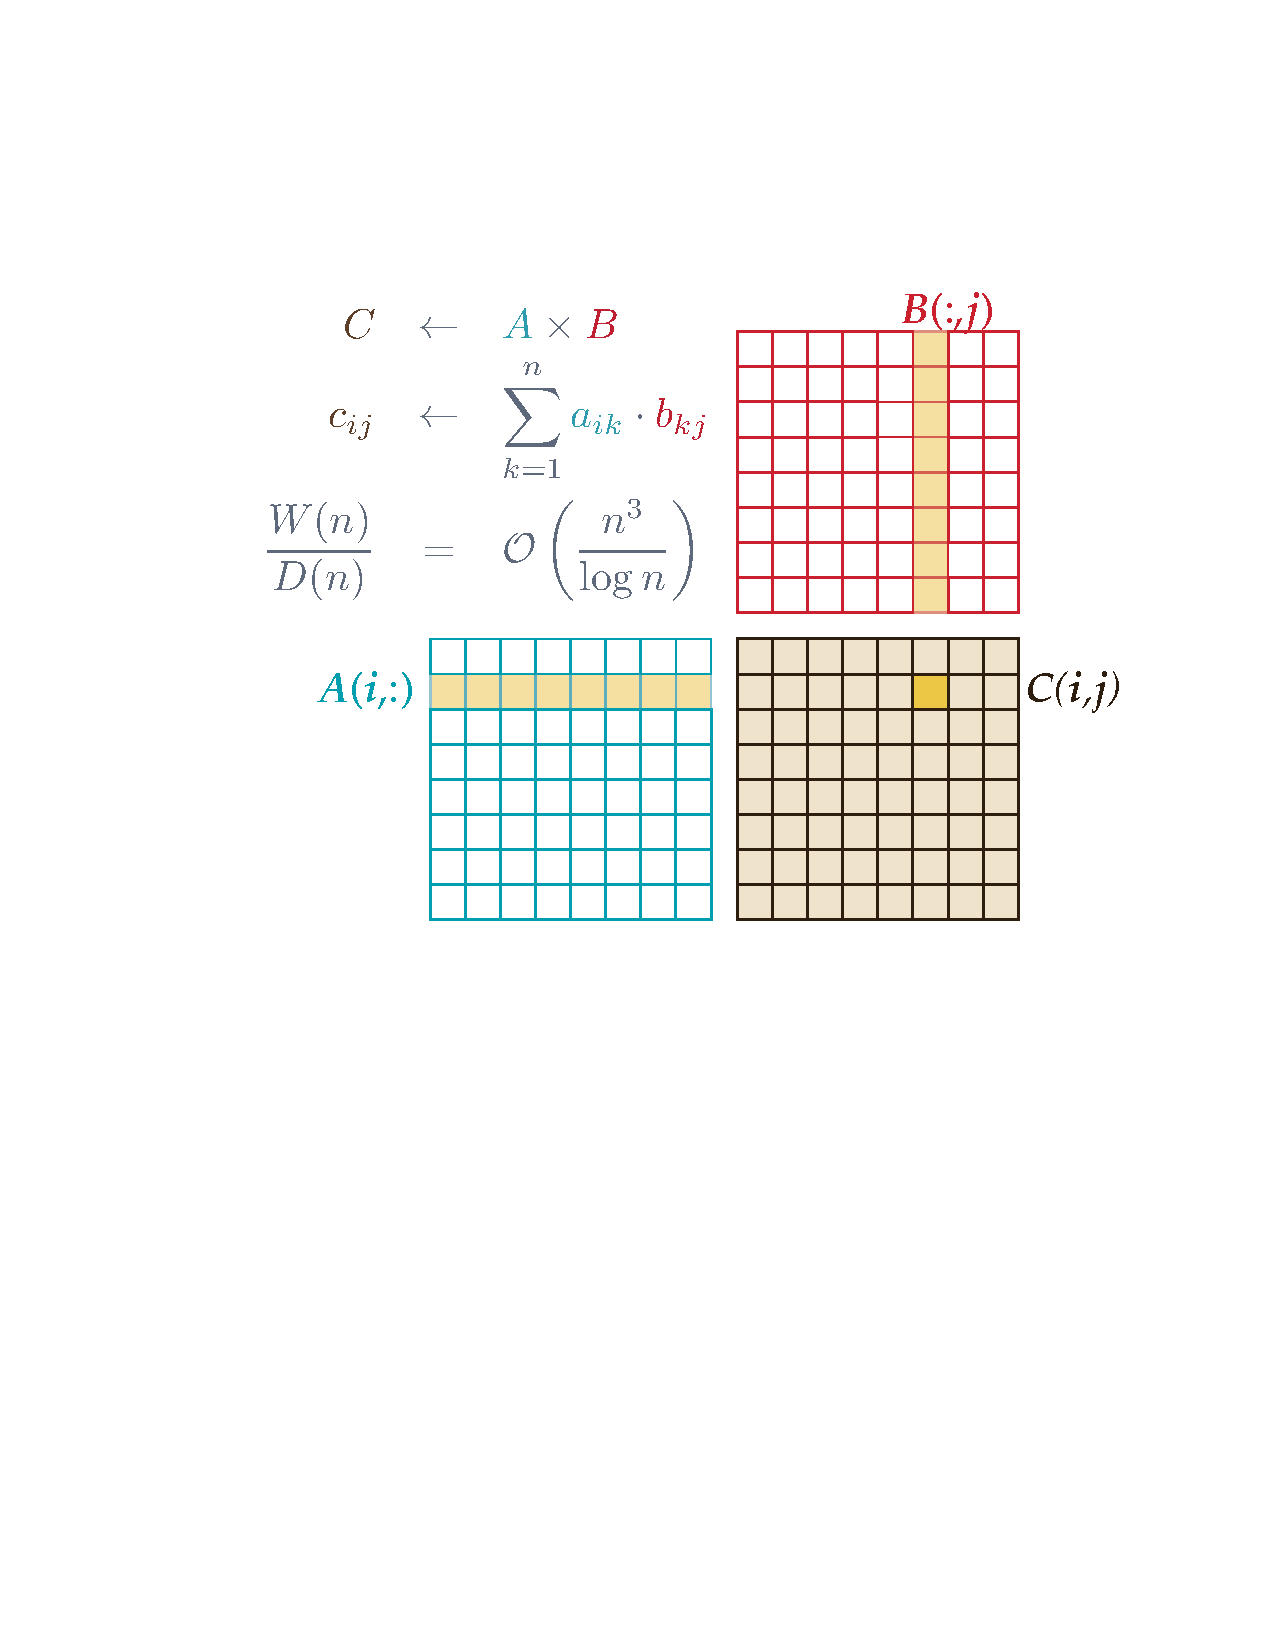
\includegraphics[width=0.49\textwidth]{matrix-work-depth.pdf}
        \caption{Work-depth example: multiplying two n × n matrices.}
        \label{fig:matrix}
\end{figure}

\noindent
\textbf{\textit{Example: Matrix multiply.}} 
Consider the multiplication of two $n × n$ matrices, $C \leftarrow A × B$, as illustrated in Figure \ref{fig:matrix}. 
Each output element $c_{ij}$ is the dot product between $A_{i,:}$, which is row $i$ of $A$, and $B_{:,j}$ , which is column $j$ of $B$. $A$ dot product involves an elementwise multiplication of the vectors, followed by a sum-reduction of those results. This dot product requires $\Theta (n)$ operations.
Since there are $n^2$ elements of $C$, the work $W(n) = \Theta(n^3)$\footnote{We assume a conventional matrix multiply, rather than an asymptotically faster algorithm, such as Strassen’s algorithm}.
To compute $D(n)$, observe that the $n^2$ output elements have no dependencies among them; the only dependencies occur during the reduction to compute each output element. Thus, $D(n) = \Theta(\log n)$. 
The ratio of $W(n)/D(n) = \Theta(n^3/\log n)$ is asymptotically very high, and so our analysis confirms what we would expect, namely, that a matrix multiply has plenty of parallelism for even modestly sized values of $n$.
\subsection{Charterizing I/O Behavior}
Besides parallelism, data movement is the other critical characteristic of an algorithm. To analyze data movement, we consider the classical \textit{external memory model}. 
\begin{figure}[htb]
        \centering
        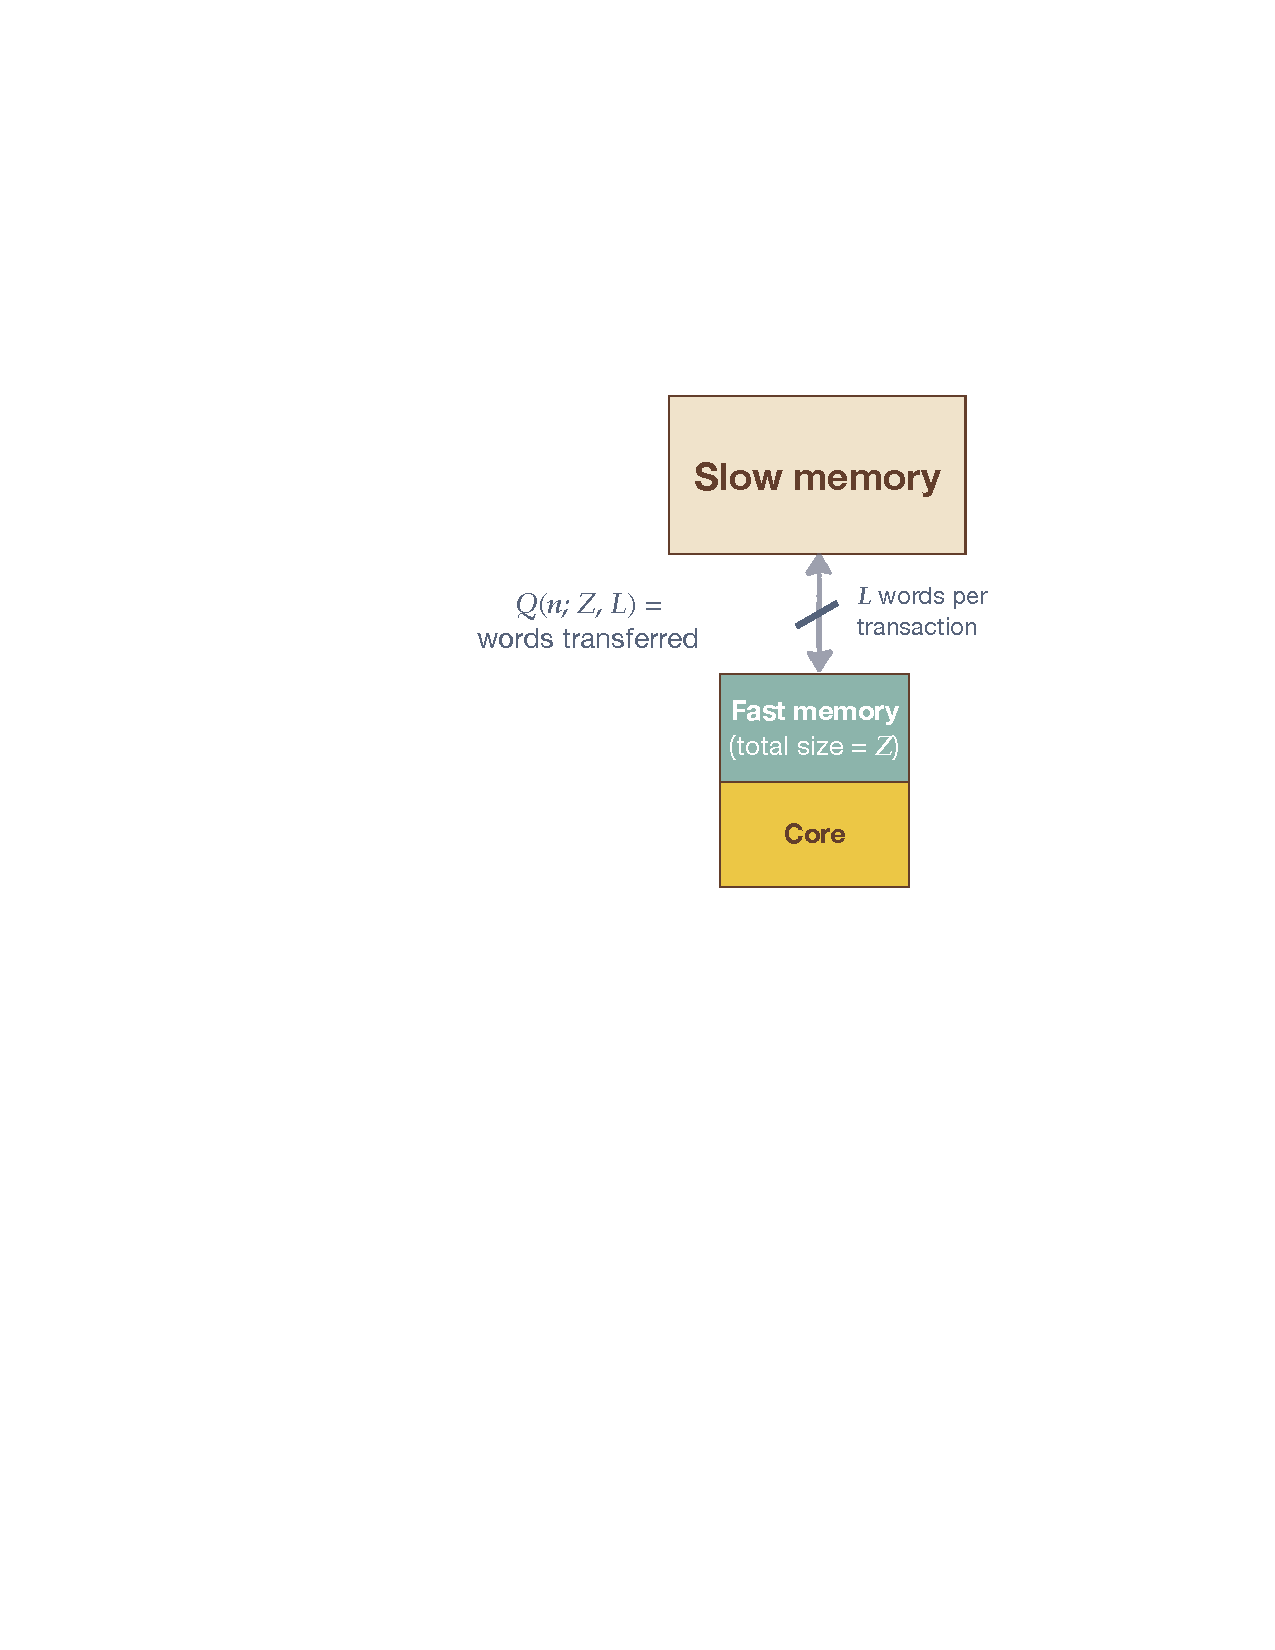
\includegraphics[width=0.3\textwidth]{abstract-machine.pdf}
        \caption{An abstract machine with a \textit{two-level memory hierarchy}. The fast memory (e.g., cache or local-store) can hold $Z$ words. Our goal is to design algorithms that, given an input of size n, are work-optimal but also minimize the number of transfers $Q(n; Z)$ between the slow and fast memories (alternatively, that are work-optimal and maximize the computational intensity, $W (n)/Q(n; Z)$).}
        \label{fig:abstract-machine}
\end{figure}

Consider first a \textit{sequential} processor with a two-level memory hierarchy consisting of a large but slow memory and a small fast memory of size $Z$ words; work operations may only be performed on data that lives in fast memory. This fast memory may be an automatic cache or a software- controlled scratchpad; our analysis here is agnostic to this choice. We may further consider that transfers between slow and fast memory must occur in discrete transactions (blocks) of size $L$ words. When we design an algorithm in this model, we again measure the work, $W (n)$; however, we also measure Q(n; Z, L), the number of L-sized transfers between slow and fast memory for an input of size n. There are several ways to design either cache-aware or cache-oblivious algorithms and then analyze $Q(n; Z, L)$. 
In either case, when we design an algorithm in this model, we again aim for work-optimality while also trying to maximize the algorithm’s \textit{computational intensity}, which is $W (n)/ (Q(n; Z, L) \cdot L)$. Intensity is the algorithmic ratio of operations performed to words transferred and, in practice, is often converted and cited as the algorithm’s “flop-to-byte” ratio.
\begin{figure}[htb]
        \centering
        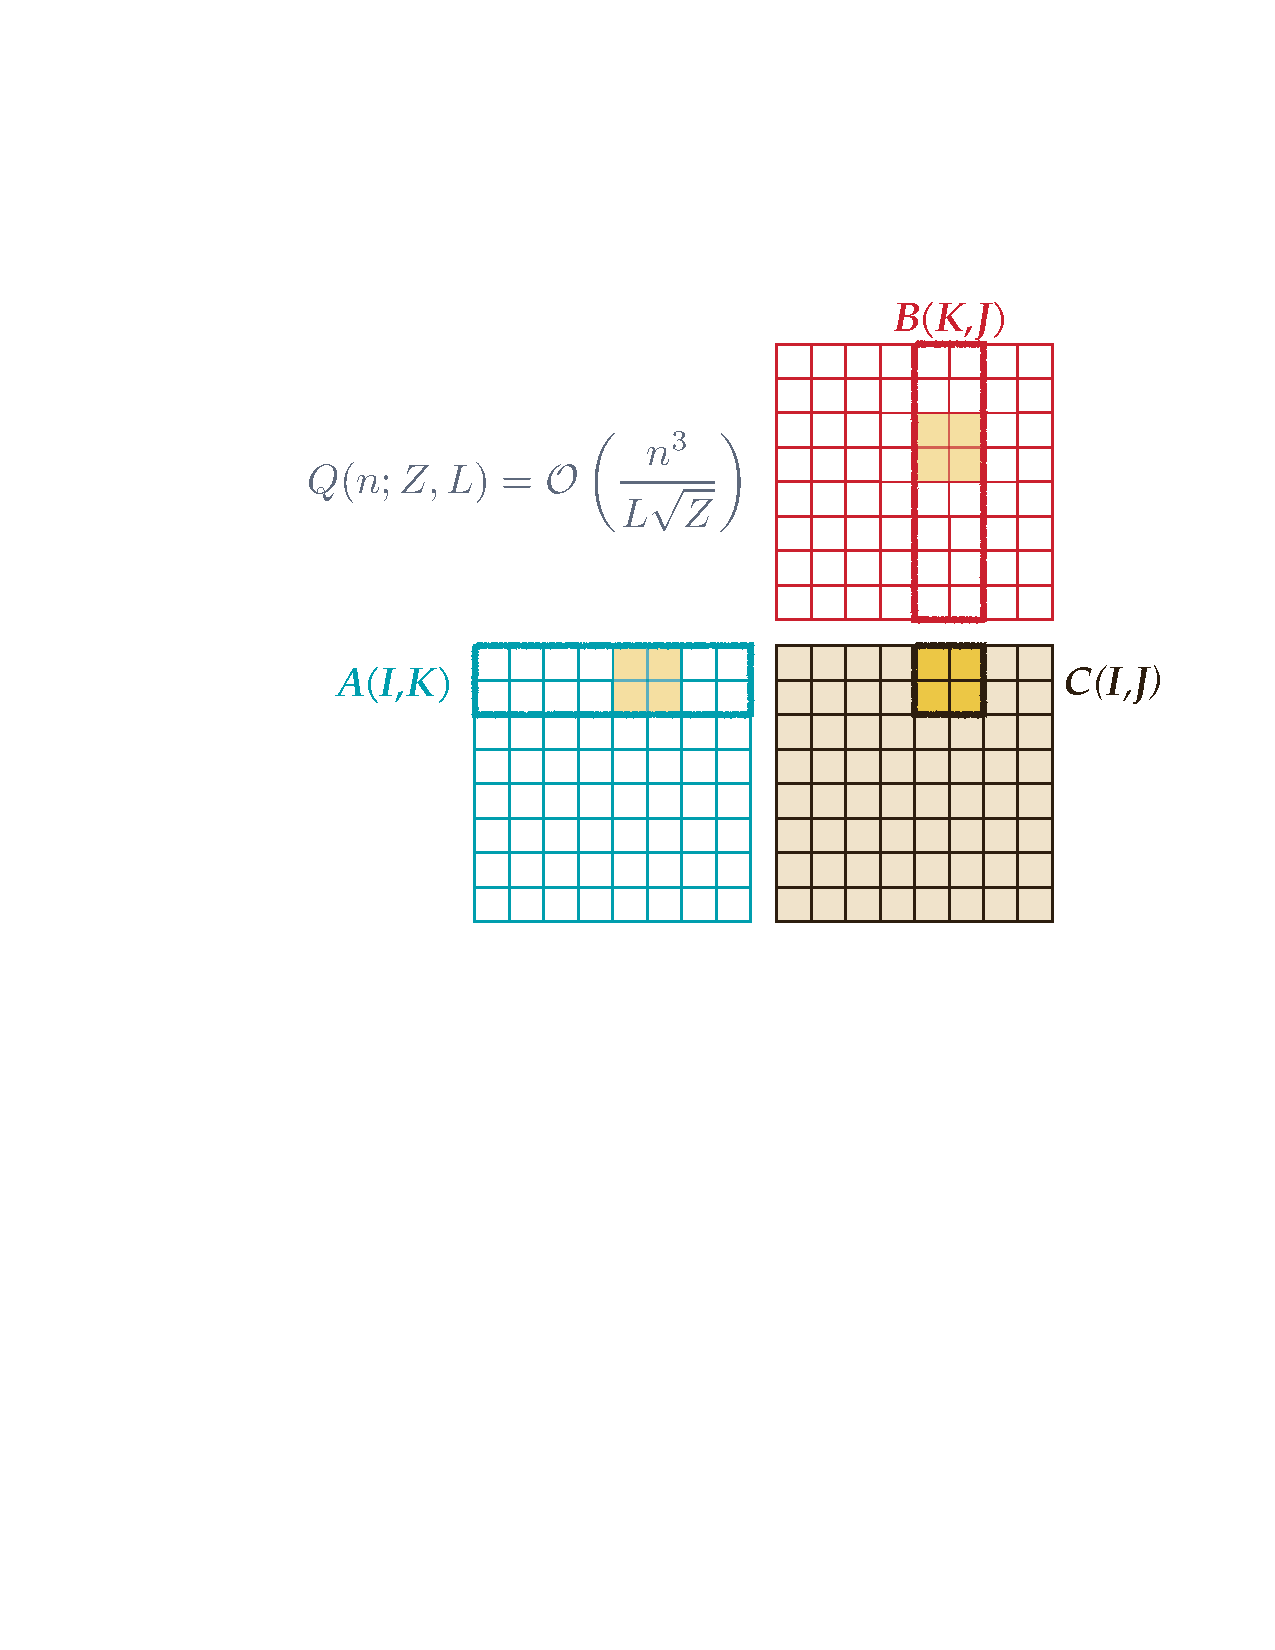
\includegraphics[width=0.49\textwidth]{block-matrix.pdf}
        \caption{A blocked matrix multiply performs $O(n^3/(L\sqrt Z))$ I/Os in the external memory model, assuming that: 
(i) each of the three blocks of $A, B,$ and $C$ needed to compute an output block of $C$ are stored contiguously; and (ii) that these three blocks just fit into the fast memory.}
        \label{fig:block-matrix}
\end{figure}

\noindent
\textbf{\textit{Example: Matrix multiply.}} 
Algorithms for conventional matrix multiply perform $W(n) = \Theta(n^3)$ operations on $ \Theta(n^2)$ words of data;
thus, a naive lower bound on $Q(n; Z, L)$ would be $\Sigma(n^2/L)$ transfers. The intensity could therefore be a high as $O(n)$.

Consider two candidate algorithms for matrix multiply. The first is the one shown in Figure \ref{fig:matrix}, which is based on performing $n^2$ reductions of length $n$ each. This algorithm results in $Q(n; Z, L) = O(n^3/L)$ transfers, assuming the preceding analysis for reductions. The intensity is therefore just $O(1)$. 
Compared to our naive estimate of $O(n)$, it is likely there is a better algorithm.

The well-known alternative appears in Figure \ref{fig:block-matrix}. 
This algorithm updates blocks of $C$ at a time, rather than a single element of $C$, 
and streams through blocks of $A$ and $B$ as shown. 
That is, the algorithm performs block updates instead of row/column dot products. In this case, if
\bi
\ii the block size is $b \times b$;
\ii three blocks can be fit in fast memory at once, i.e., $3b^2 \leq Z$; and
\ii blocks are stored contiguously, so that just $b^2/L$ transfers are required to load a block,
\ei
then it can be shown that $Q(n; Z, L) = O(n^3/(L \sqrt{Z}))$.
Therefore, the intensity is $O(\sqrt{Z})$.
If $Z=\Omega(L^2)$, the intensity of this algorithm is much higher than that of the naive algorithm. In practice, a local-store or cache size $Z$ is typically much larger than corresponding minimum transfer or line size $L$, so this assumption is likely to hold\footnote{An exception to this rule is a TLB, which for typical configurations is like a cache with very large lines and having a capacity of a small number of lines.}.

One might reasonably ask whether this value of $Q(n; Z, L)$ can be improved upon further, given our naive lower-bound estimate of $O(n^2)$.
For general matrices and the conventional matrix multiply algorithm, the answer is that no algorithm can move fewer words than the blocked algorithm -- the blocked algorithm is asymptotically optimal.
So-called \textit{cache-oblivious} approaches also only match this bound.

\noindent
\textit{\textbf{A few summary observations about I/O.}} 
The case of I/O analysis is evidently more complex than the analysis of parallelism in the following ways.
\bi
\ii The I/O analysis is not independent of the machine parameters, the way the work-depth analysis was independent of the number of processors, $p$.
\ii The two example I/O analyses both included assumptions of \textit{contiguous layouts}. 
That is, inclusion of the parameter, $L$, forces the algorithm designer to take data layout into account.
\ii Recall that for matrix multiply, we were able to state a \textit{lower bound} on the number of I/O transfers for \textit{any} algorithm. This is one area in which theoretical analysis, when further refined to account for additional architectural details, can provide insights into performance that are difficult to extract from code or benchmarks.
\ei

In addition, we might ask what the relative asymptotic pay-off from increasing hardware memory resources
 (e.g., $Z$ and $L$) is relative to increasing hardware parallelism (e.g., $p$). 
For example, for compute-rich matrix multiply, we see that doubling $Z$ yields a $\sqrt{2}$ reduction in I/Os, whereas doubling $L$ cuts I/Os in half. Then, if the cost of doubling $Z$ and doubling $L$ are equal, it would be more cost effective to double $L$. This analysis confirms an intuition behind GPU design of favoring significant increases in memory-level parallelism (larger $L$) over bigger caches (larger $Z$).

\subsection{Abstract and Concrete Measures}
Work, depth, and the number of I/Os or cache misses are all abstract quantities, whereas the ultimate goal—-if it is possible—-would be to make stronger statements about execution time and time- scalability. Such a time-based analysis minimally requires an architectural cost model. If we are able to do so, what would the theory tell us?

Consider an example of the generic manycore processor system shown in Figure \ref{fig:manycore}. 
This system has $p$ cores, each of which can deliver a maximum of $C_0$ operations per unit time; a fast memory of total size $Z$ words, partitioned among the cores; and a memory system whose cost to transfer $m \cdot L$ words is $\alpha + m \cdot L/\beta$, where $\alpha$ is the latency and $\beta$ is the bandwidth in units of words per unit time\footnote{This abstract machine is intended to very coarsely approximate an NVIDIA Fermi-class architecture, where $Z$ might represent the aggregate register and multiprocessor-private first-level local-store and cache capacity.}.
\begin{figure}[htb]
        \centering
        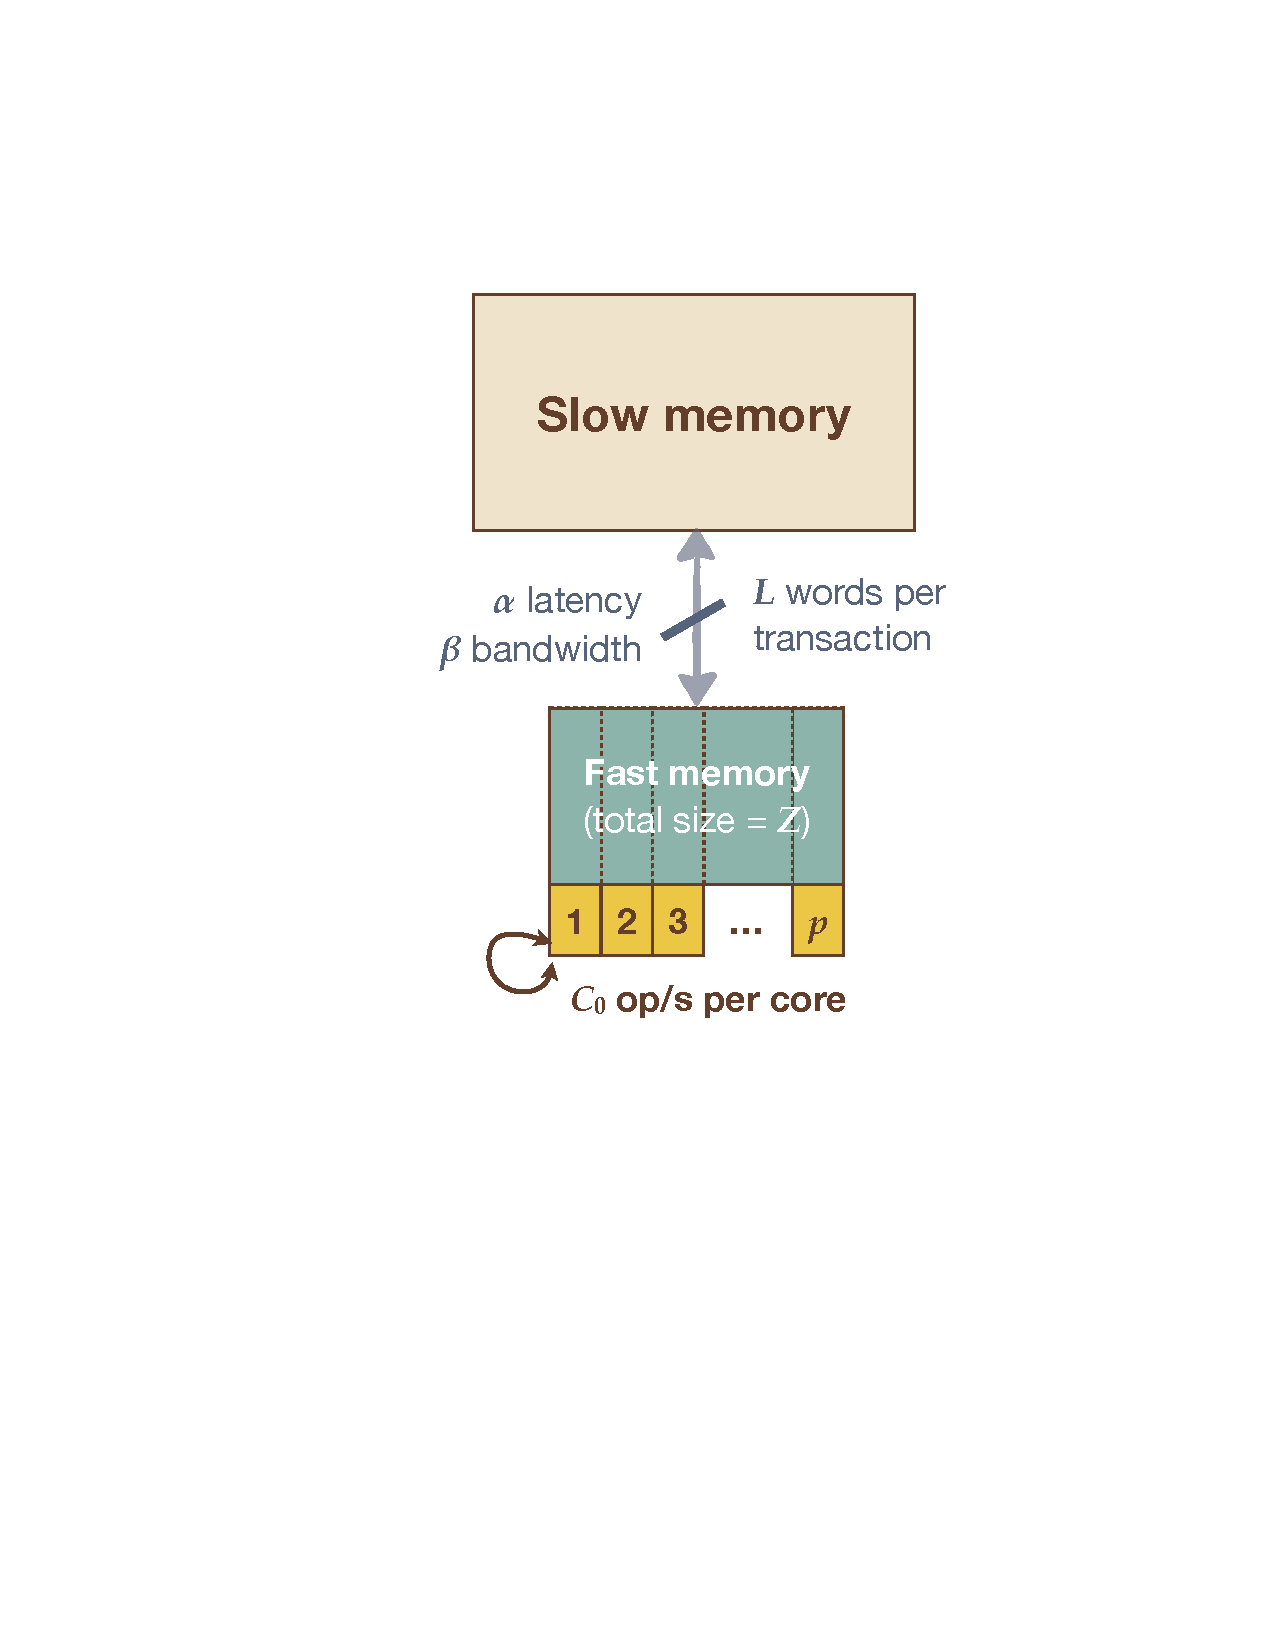
\includegraphics[width=0.25\textwidth]{manycore-processor.pdf}
        \caption{An abstract manycore processor with $p$ cores, each with a peak execution rate of $C_0$ operations per unit time; an aggregate fast memory capacity of $Z$ words partitioned among the cores; and a channel between slow and fast memory such with latency α time units, bandwidth $\beta$ words per unit time, and minimum transaction size $L$ words.}
        \label{fig:manycore}
\end{figure}

Equation \ref{eqn:cost} gives us a way to estimate the time, $T_{comp}(n; p)$, just to complete the computational work for this system. To estimate the I/O time, $T_{mem}(n)$, suppose we know $Q_p(n; Z, L)$ and charge the full latency $\alpha$ for each enode on the critical path. 
Let us further assume that all $Q_p(n; Z, L)$ memory transfers will in the best case be aggregated and pipelined by the memory system and thereby de delivered at the peak bandwidth, $\beta$. Then,
\begin{equation}
T_{mem}(n; p, Z, L, \alpha, \beta) = \alpha \cdot D(n) + \frac{Q_p(n; Z, L)(n) \cdot L}{\beta}
\end{equation}
This cost model is not definitive, but sufficient to illustrate a few points.
 \section{Exploring the Design Space}
\subsection{Design Space of a GPU-Aware DBMS Architecture}
In this section, we explore the design space of a GPU-accelerated database management system (GDBMS). 
GDBMSs should be \textit{in-memory column stores}, should use the \textit{block- at-a-time processing model }and exploit all available processing devices for query processing by using a \textit{GPU-aware query optimizer}.
 Thus, main memory DBMSs are similar to GPU-accelerated DBMSs, and most in-memory, column-oriented DBMSs can be extended to efficiently support co-processing on GPUs.
\begin{figure}[htb]
        \centering
        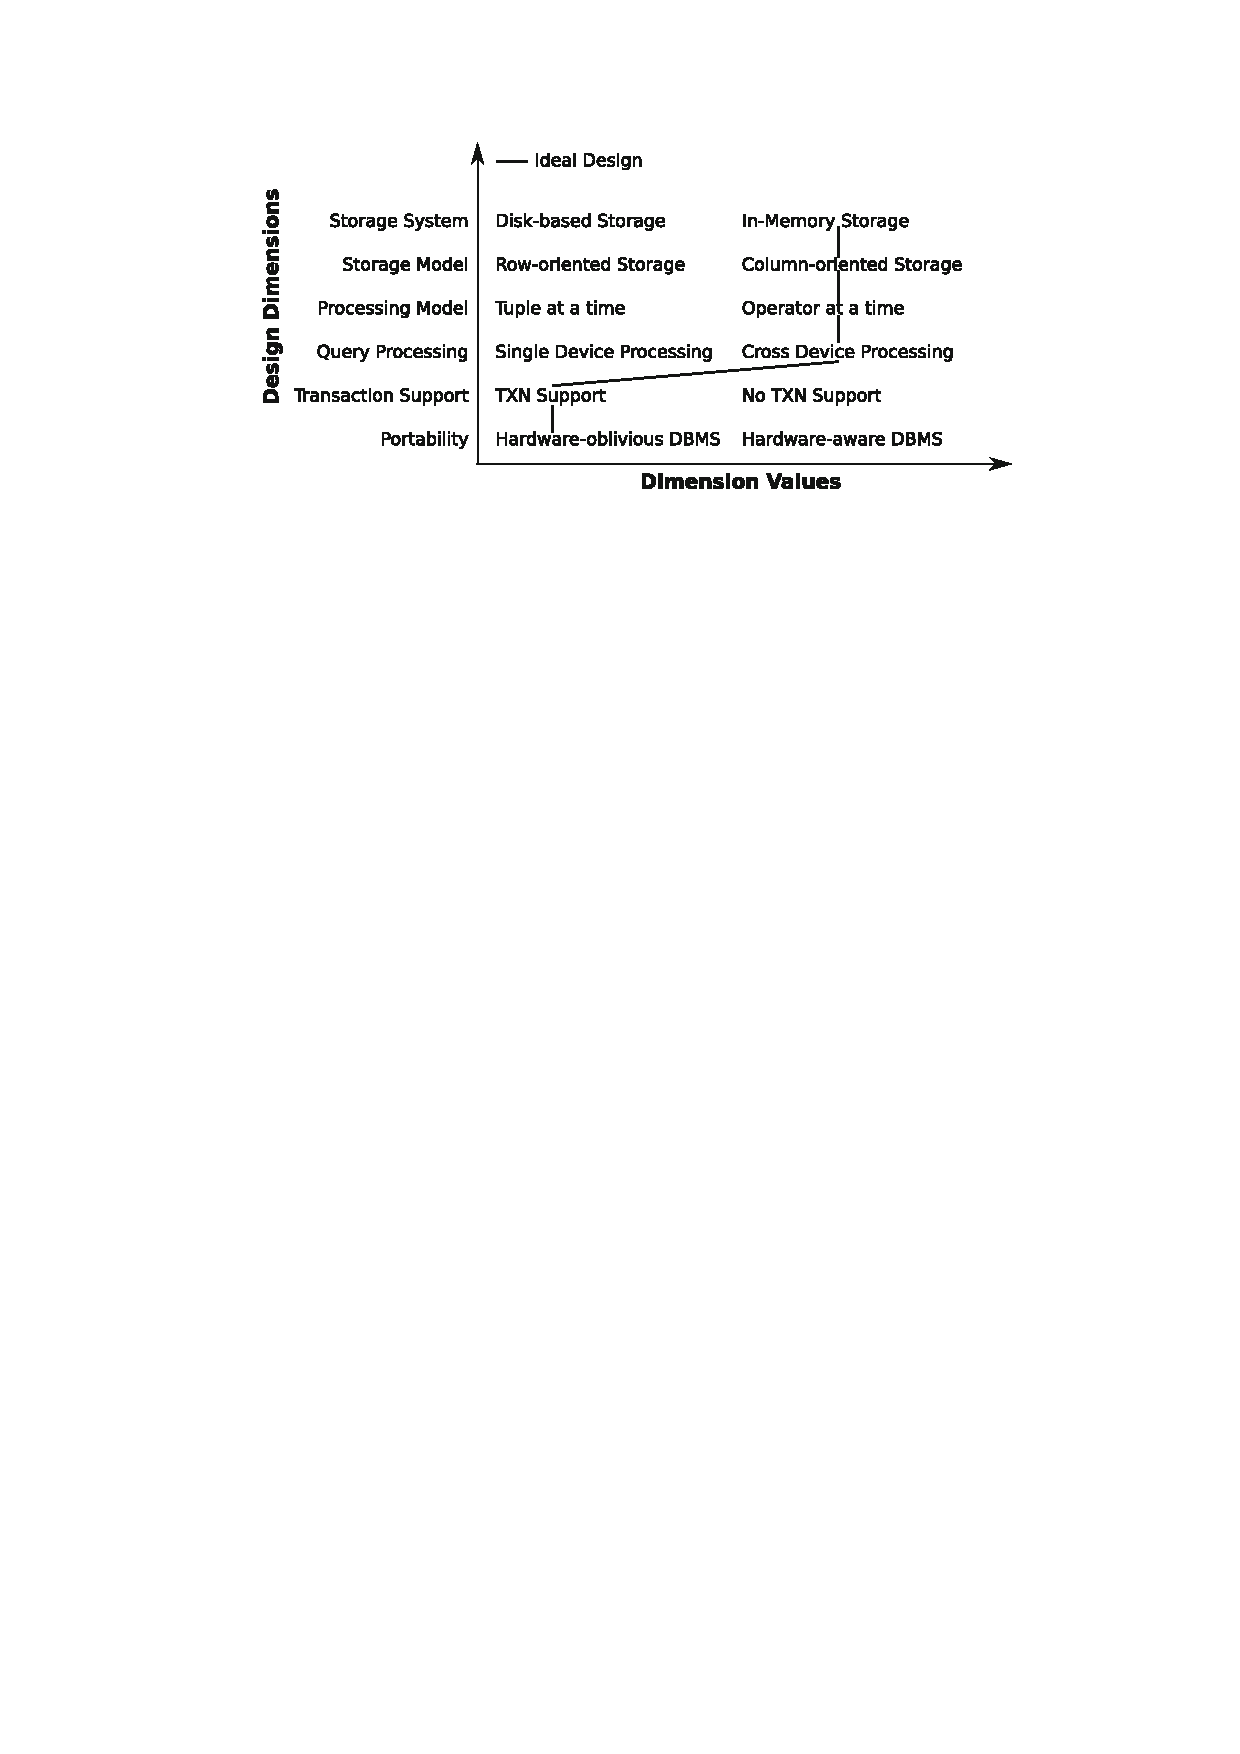
\includegraphics[width=0.48\textwidth]{design-space.pdf}
        \caption{Design space of GPU-aware DBMSs}
        \label{fig:design-space}
\end{figure}
Figure \ref{fig:design-space} shows the design space of a GPU-aware DBMSs.
A GPU-aware database system should reside \textit{in-memory} and use \textit{columnar storage}. 
As processing model, it should implement \textit{operator-at-a-time} bulk processing model \cite{Manegold:2009}, potentially enhanced by dynamic code compilation. 
The system should make use of all available (co-)processors in the system (including the CPU!) by having a locality-aware query optimizer, which distributes the workload across all available processing resources. In case the GPU-aware DBMS needs transaction sup- port, it should use an optimistic transaction protocol, such as the timestamp protocol. Finally, in order to reduce implementation overhead, the ideal GDBMS would be hardware-oblivious, meaning all hardware-specific adaption is handled transparently by the system itself.

\section{A Survey of GDBMSs}
In this section, we refine our theoretical discussion of the GDBMS design space.
We identified the following \textit{eight} academic systems that are relevant for our survey; CoGaDB, GPUDB, GPUQP, GPUTx, MapD, Ocelot, OmniDB, and Virginian \cite{gpgpu:2014}. We present for each GDBMS the storage system, the \textit{storage} and \textit{processing} model, \textit{query placement} and \textit{query optimization}, and support for \textit{transaction} processing.

\subsection{CoGaDB}
CoGaDB\footnote{ Source code available at: \href{http://wwwiti.cs.uni-magdeburg.de/iti db/research/gpu/cogadb/}{http://wwwiti.cs.uni-magdeburg.de/iti db/research/gpu/cogadb/}.} focuses on GPU-aware query optimization to achieve efficient co-processor utilization during query processing \cite{BreB:2013, seb:2013}. Figure \ref{fig:cogadb} shows the architecture of CoGaDB.

\noindent
\textit{Storage System:} 
CoGaDB persists data on disk, but loads the complete database into main memory on startup. If the database is larger than the main memory, CoGaDB relies on the operating system’s virtual memory management to swap the least recently used memory pages on disk.

\noindent
\textit{Storage Model:}
 CoGaDB stores data in data structures optimized for in-memory databases. Hence, it stores the data column-wise and compresses VARCHAR columns using dictionary encoding. Furthermore, the data has the same for- mat when stored in the CPU’s or the GPU’s memory.

\noindent
\textit{Processing Model:} CoGaDB uses the operator-at-a-time bulk processing model to make efficient use of the memory hierarchy. This is the basis for efficient query processing using all processing resources.

\noindent
\textit{Query Placement \& Optimization:} CoGaDB uses the \textit{Hybrid Query Processing Engine} (HyPE) as physical optimizer \cite{BreB:2013, BreB:2014}. HyPE optimizes physical query plans to increase inter-device parallelism by keeping track of the load condition on all (co-)processors (e.g., the CPU or the GPU).

\noindent
\textit{Transactions:} Not supported.
\begin{figure}[htb]
        \centering
        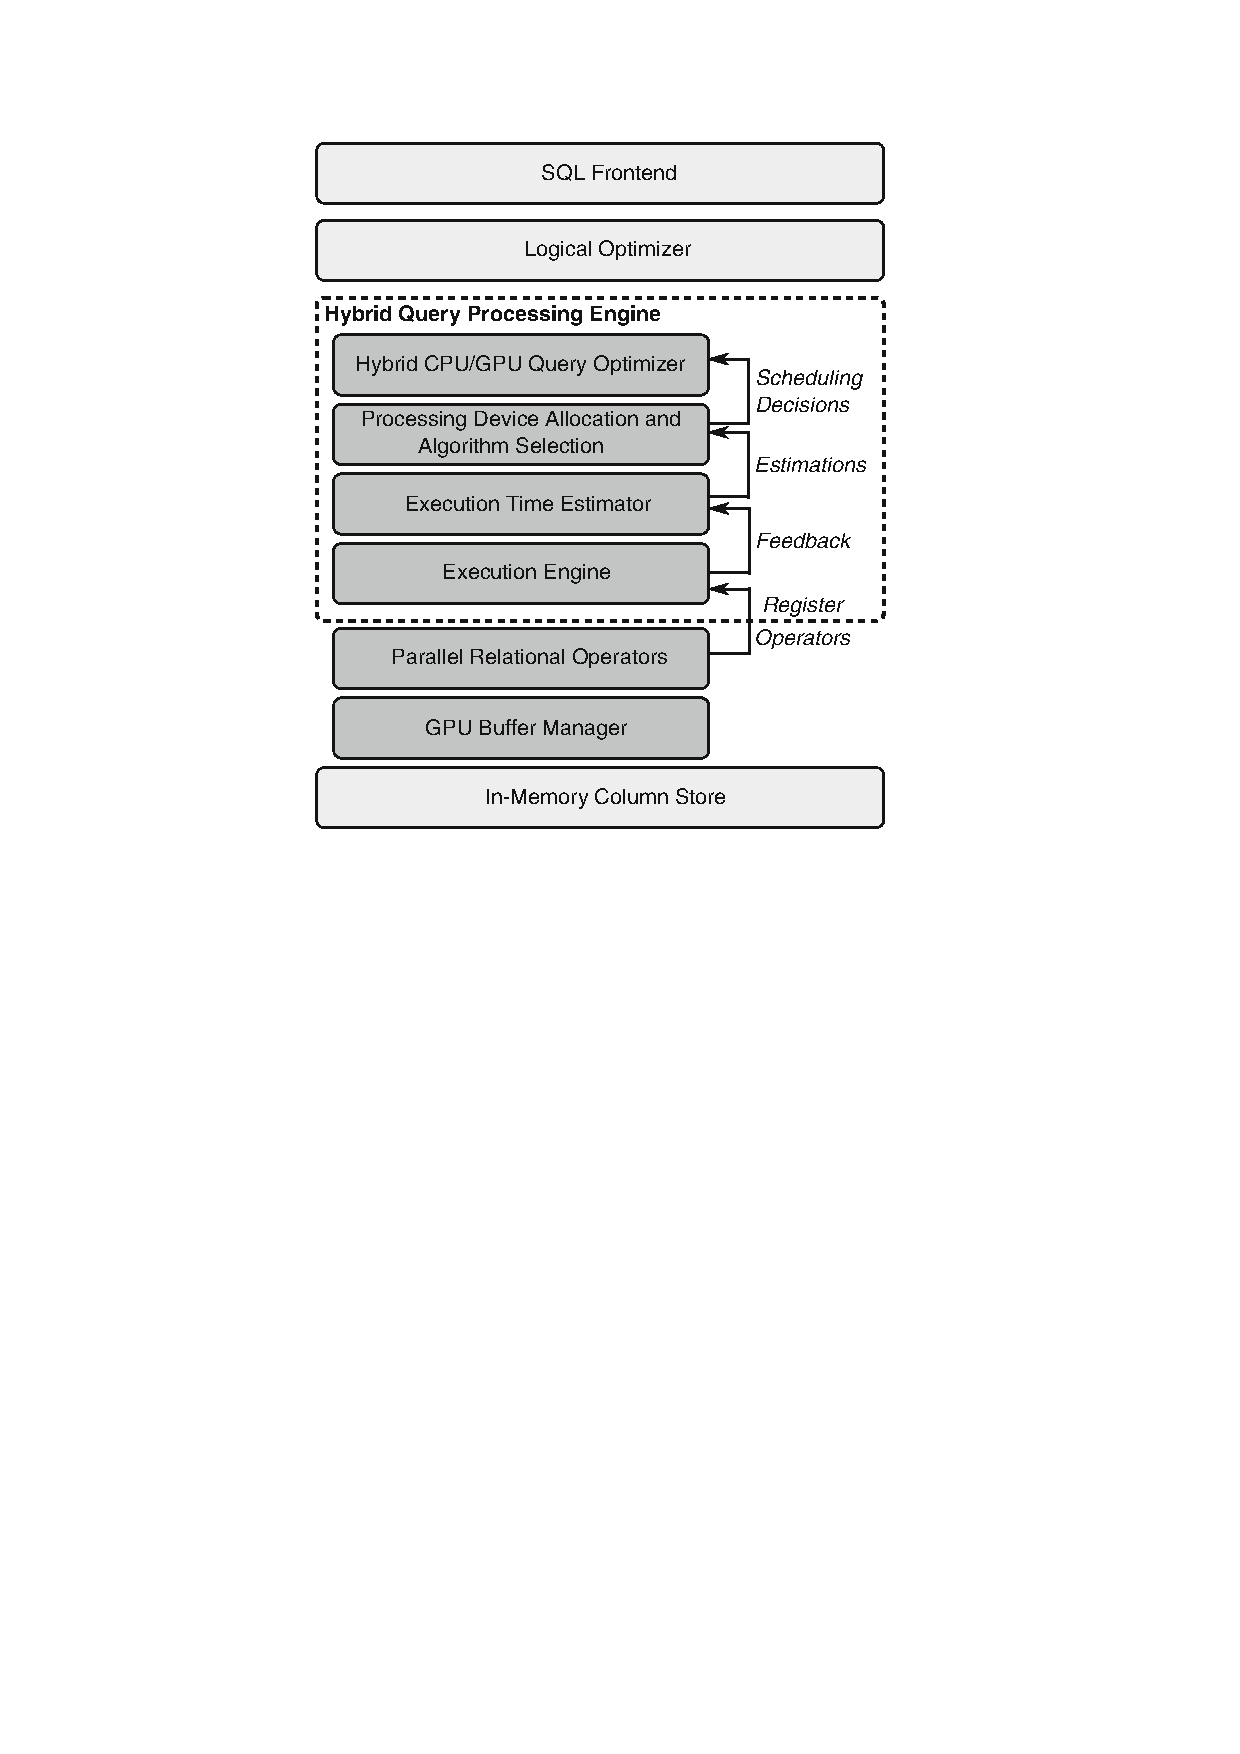
\includegraphics[width=0.48\textwidth]{cogadb.pdf}
        \caption{The architecture of CoGaDB}
        \label{fig:cogadb}
\end{figure}

\subsection{GPUDB}
In order to study the performance behaviour of OLAP queries on GPUs, Yuan and others developed GPUDB\footnote{Source code available at: \href{https://code.google.com/p/gpudb/}{https://code.google.com/p/gpudb/}.} \cite{Yuan:2013} (Fig. \ref{fig:gpudb}).

\noindent
\textit{Storage System:} 
GPUDB keeps the database in the CPU’s main memory to avoid the hard-disk bottleneck. Yuan and others identified a crucial optimization for main-memory DBMS with respect to GPU accelerated execution: In case data is stored in pinned host memory, query execution times can significantly improve (i.e., Yuan and others observed speedups up to 6.5x for certain queries of the \textit{Star Schema Benchmark} (SSB) \cite{Rabl:2013}).

\noindent
\textit{Storage Model:}
 GPUDB stores the data column-wise because GPUDB is optimized for warehousing workloads. Additionally, GPUDB supports common compression techniques (run length encoding, bit encoding, and dictionary encoding) to decrease the impact of the PCIe bottleneck and to accelerate data processing.
\begin{figure}[htb]
        \centering
        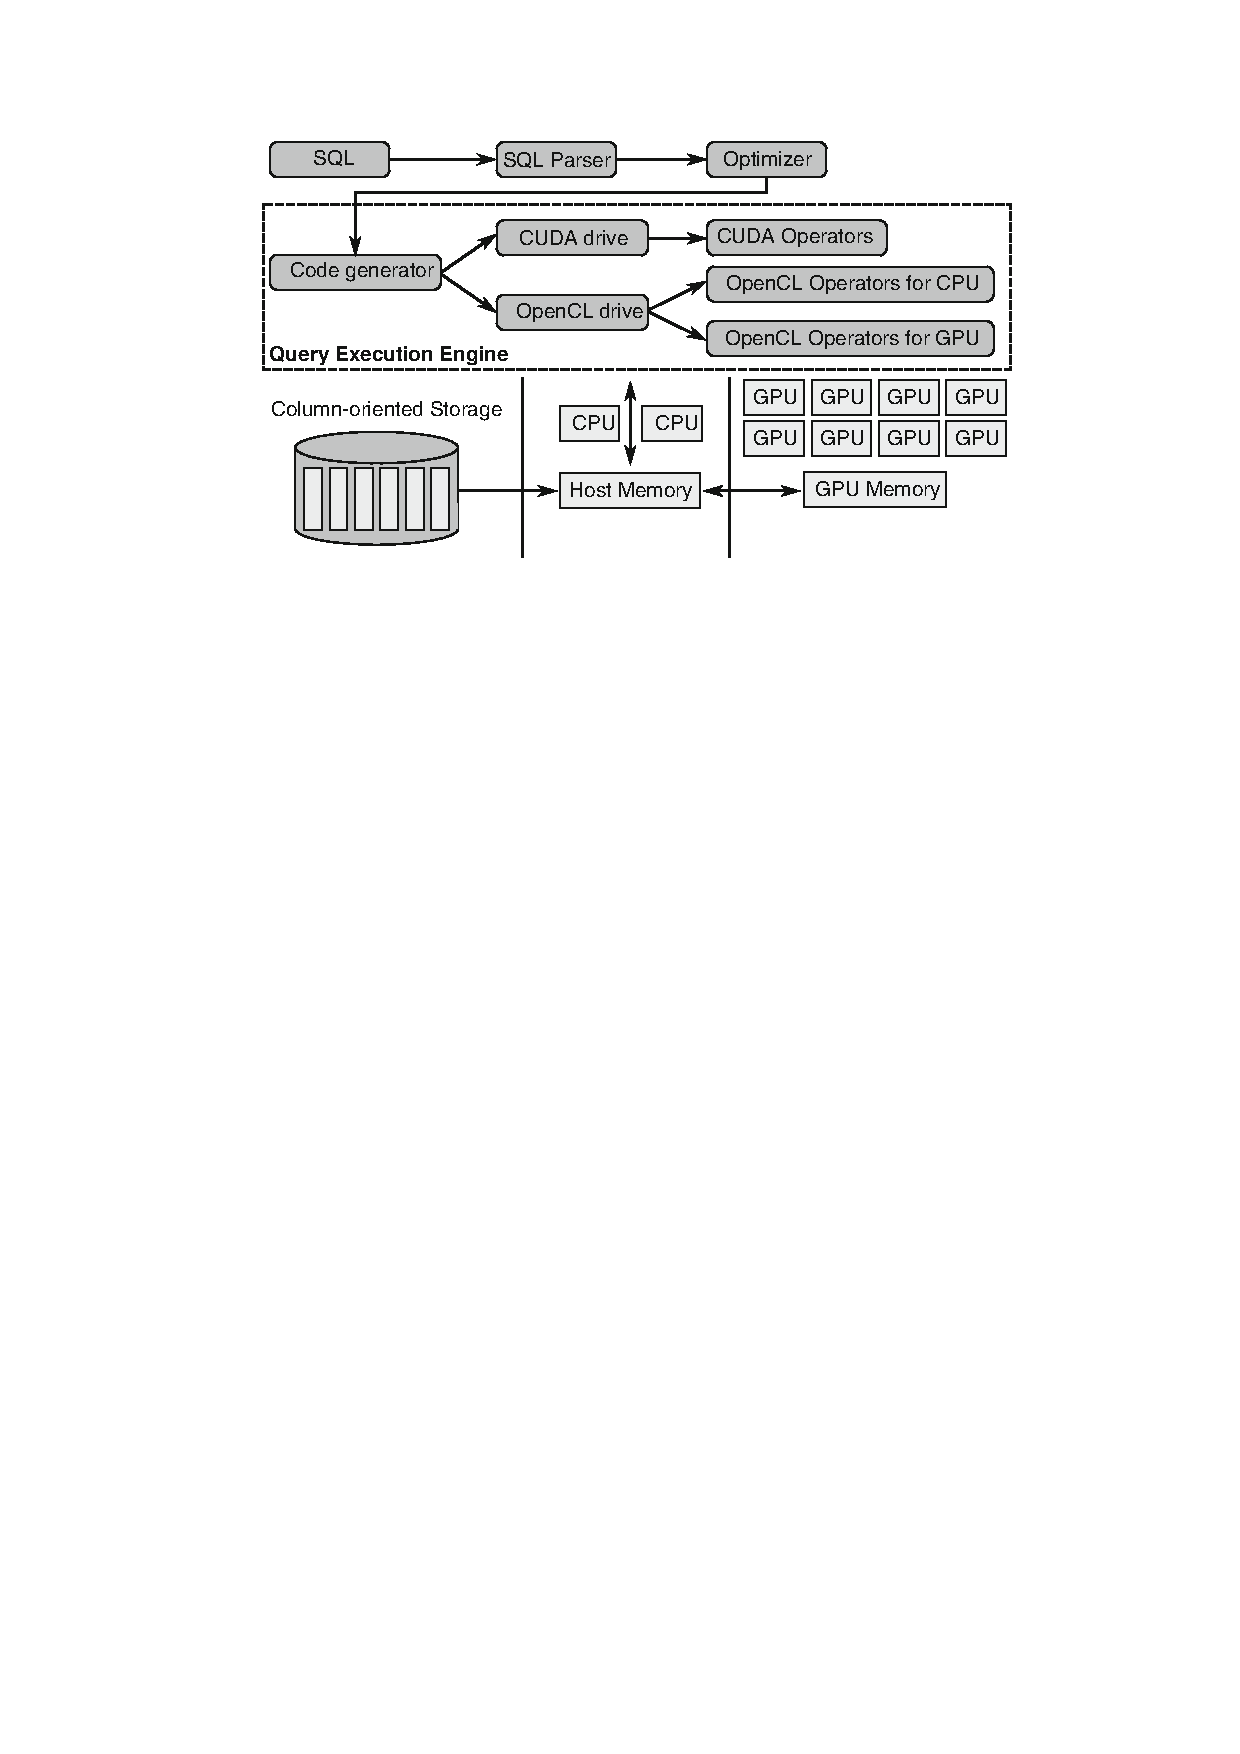
\includegraphics[width=0.48\textwidth]{gpudb.pdf}
        \caption{GPUDB: Query engine architecture}
        \label{fig:gpudb}
\end{figure}

\noindent
\textit{Processing Model:}
GPUDB uses a \textit{block-oriented processing} model: Blocks are kept in GPU RAM until they are completely processed. This processing model is also known as \textit{vectorized processing}. Thus, the PCIe bottleneck can be further reduced by overlapping data transfers with computation. For certain queries, Yuan and others observed speedups up to 2.5x compared to no overlapping of processing and data transfers.

GPUDB compiles queries to \textit{driver programs}. A driver program executes a query by calling pre-implemented GPU operators. Hence, GPUDB executes all queries on the GPU and the CPU performs only dispatcher and post processing tasks (i.e., the CPU is used less than 10\% of the time during processing SSB queries \cite{Yuan:2013}).

\noindent
\textit{Query Placement \& Optimization:} GPUDB has no support for executing queries on the CPU and GPU in parallel.

\noindent
\textit{Transactions:} Not supported.


\subsection{GPUQP}
He and others developed GPUQP\footnote{Source code available at: \href{http://www.cse.ust.hk/gpuqp/}{http://www.cse.ust.hk/gpuqp/}.}, a relational query processing system, which stores data in-memory and uses the GPU to accelerate query processing \cite{Fang:2007}. In GPUQP, each relational operator can be executed on the CPU or the GPU (Fig. 6).

\noindent
\textit{Storage System:} 
GPUQP supports in-memory and disk-based processing. 
Apparently, GPUQP also attempts to keep data cached in GPU memory. 
Unfortunately, the authors do not provide any details about the used data placement strategy.

\noindent
\textit{Storage Model:} 
Furthermore, GPUQP makes use of columnar storage and query processing, which fits the hardware capabilities of modern CPUs and GPUs.
\begin{figure}[htb]
        \centering
        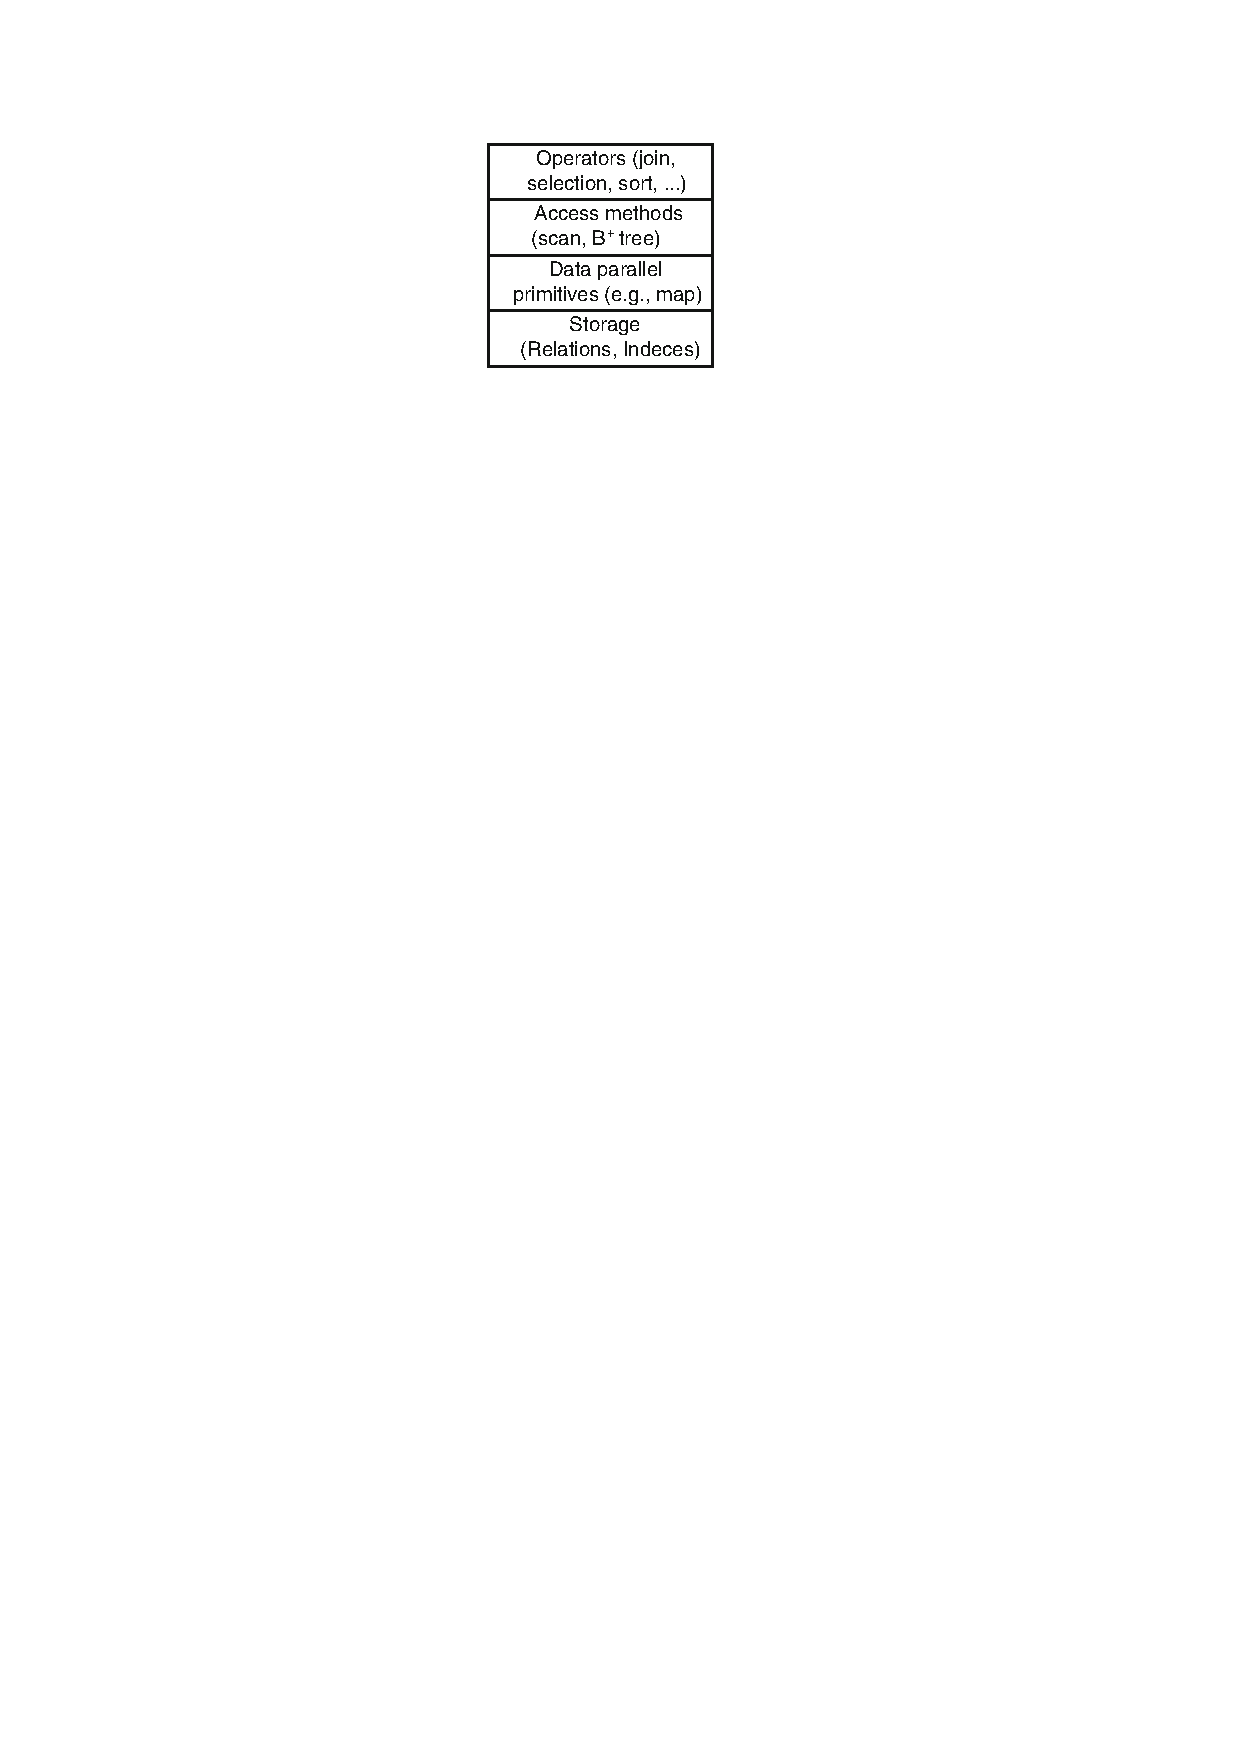
\includegraphics[width=0.2\textwidth]{gpuqp.pdf}
        \caption{Execution engine of GPUQP}
        \label{fig:gpudb}
\end{figure}

\noindent
\textit{Processing Model:} 
GPUQP's basic processing strategy is operator-at-a-time bulk processing. 
However, GPUQP is also capable of partitioning data for one operator and execute the operator on the CPU and the GPU concurrently. 
Nevertheless, the impact on the overall performance is small \cite{He:2009}.

\noindent
\textit{Query Placement \& Optimization:} 
GPUQP combines a Selinger-style optimizer \cite{Selinger:1988} with an analytical cost model to select the cheapest query plan. For each operator, GPUQP allocates either the CPU, the GPU, or both processors (partitioned execution). The query optimizer splits a query plan to multiple sub-plans containing at most ten operators. For each sub-query, all possible plans are created and the cheapest sub-plan is selected. Finally, GPUQP combines the sub-plans to a final physical query plan.

He and others focus on optimizing single queries and do not discuss multi- query optimization. Furthermore, load-aware query scheduling is not considered and there is no discussion of scenarios with multiple GPUs.

\noindent
\textit{Transactions:} Not supported.

\subsection{GPUTx}
In order to investigate relational transaction processing on GPUs, He and others developed GPUTx, a transaction processing engine that runs on the GPU \cite{He:2011}.

\noindent
\textit{Storage System \& Model:}
GPUTx keeps all OLTP data inside the GPU’s memory to minimize the impact of the PCIe bottleneck. 
It also applies a columnar data layout to fit the characteristics of modern GPUs.

\noindent
\textit{Processing Model:} The processing model is not built on relational operators as in GPUQP. Instead, GPUTx executes pre-compiled stored procedures, which are grouped into one GPU kernel. Incoming transactions are grouped in bulks, which are sets of transactions that are executed in parallel on the GPU.

\noindent
\textit{Query Placement \& Optimization:}
Since GPUTx performs the complete data processing on the GPU, query placement approaches are not needed.

\noindent
\textit{Transactions:}
GPUTx is the only system in our survey – and that we are aware of – that supports running transactions on a GPU. It implements three basic transaction protocols: \textit{Two-phase locking}, \textit{partition-based execution} and $k$\textit{-set- based execution}. The major finding of GPUTx is that \textit{locking-based} protocols do not work well on GPUs. 
Instead, \textit{lock-free} protocols such as partition-based execution or $k$-set should be used.

\subsection{MapD}
Mostak develops MapD (\textit{Massively Parallel Database}), which is a data processing and visualization engine, combining traditional query processing capabilities of DBMSs with advanced analytic and visualization functionality \cite{mapd:2015}. 
One application scenario is the visualization of twitter messages on a road map\footnote{\href{http://mapd.csail.mit.edu/tweetmap/}{http://mapd.csail.mit.edu/tweetmap/}.}, in which the geographical position of tweets is shown and visualized as heat map.
\begin{figure}[htb]
        \centering
        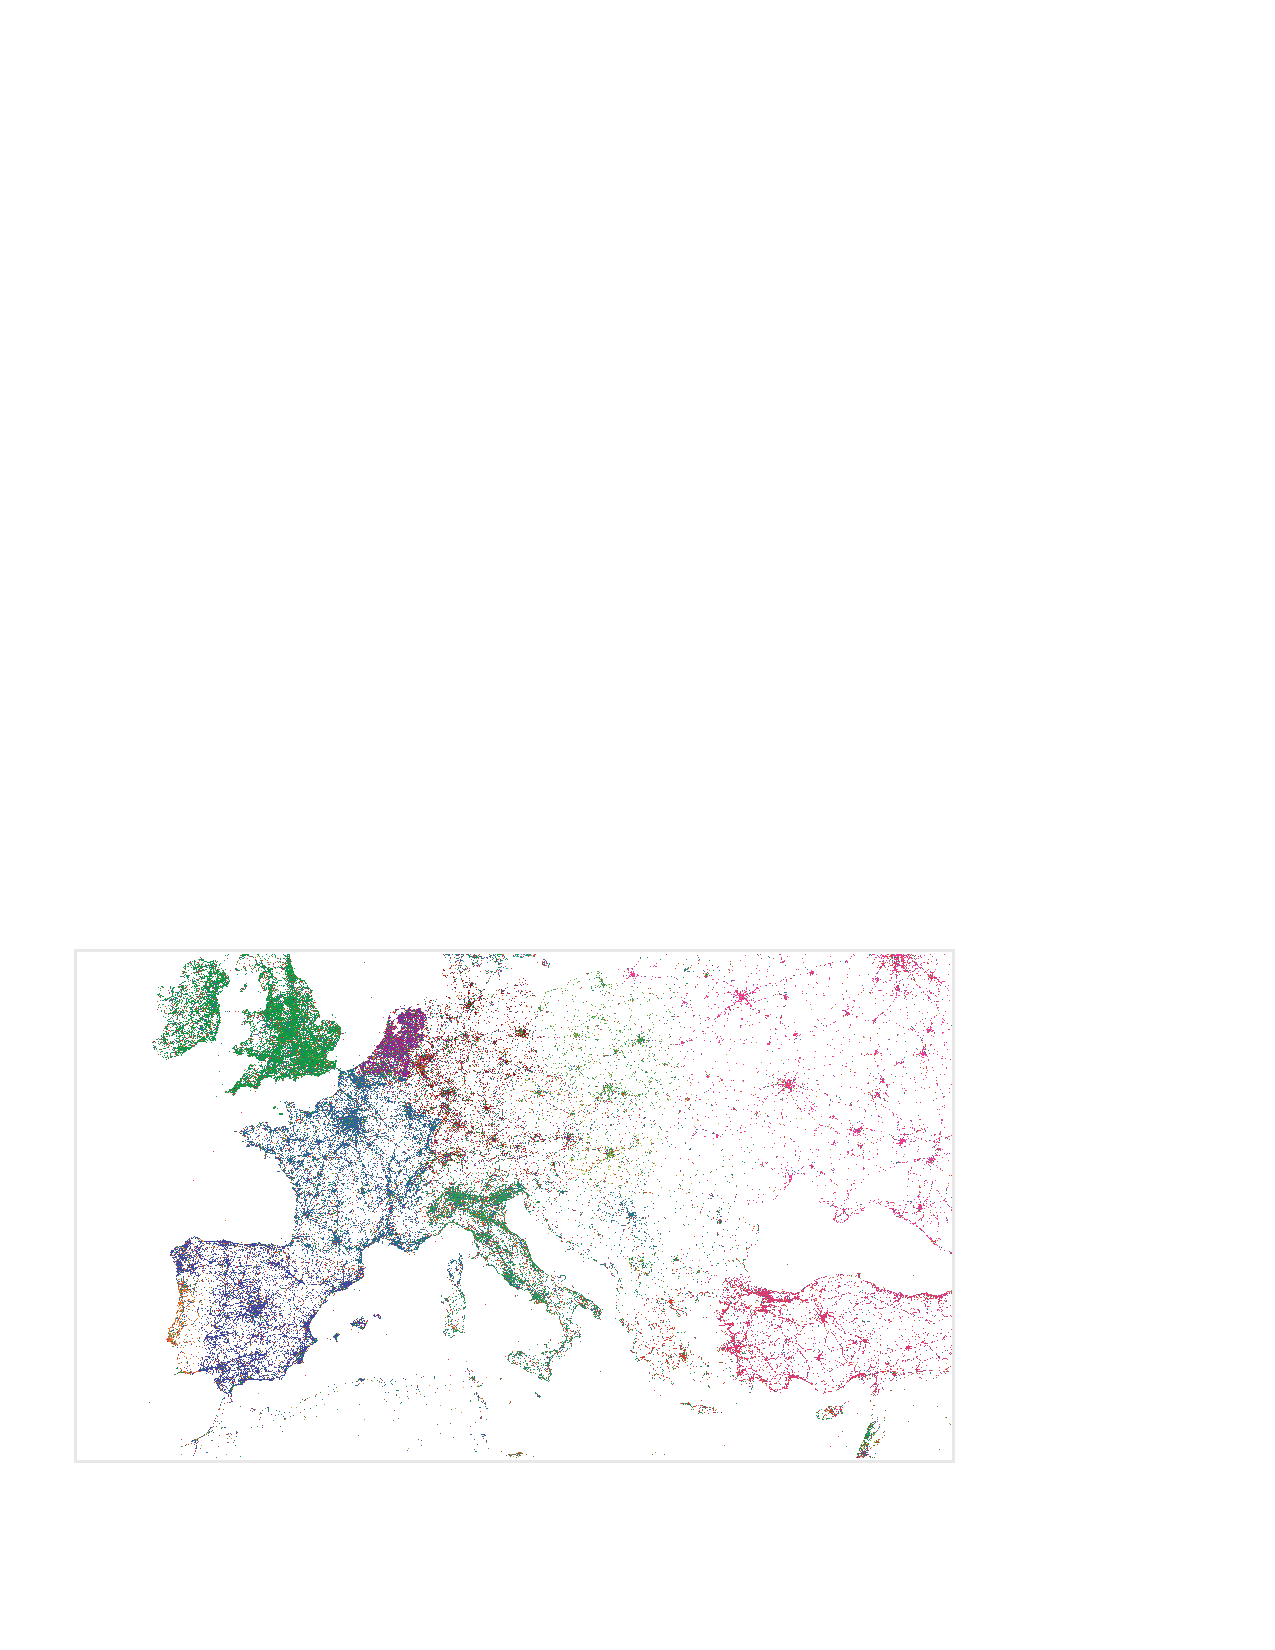
\includegraphics[width=0.49\textwidth]{mapd-visualization.pdf}
        \caption{A MapD-rendered visualization of 500 million tweets in Europe colored by language used.}
        \label{fig:mapd-visualization}
\end{figure}

\noindent
\textit{Storage System:} The data processing component of MapD is a relational DBMS, which can handle data volumes that do not fit the main memory. MapD also tries to keep as much data in-memory as possible to avoid disk accesses.

\noindent
\textit{Storage Model:} 
MapD stores data in a columnar layout, and further partitions columns into \textit{chunks}. 
A chunk is the basic unit of MapD's memory manager. 
The basic processing model of MapD is processing one \textit{operator-at-a-time}. 
Due to the partitioning of data into chunks, it is also possible to process on a per- chunk basis. Hence, MapD is capable of applying \textit{block-oriented} processing.

\begin{figure}[htb]
        \centering
        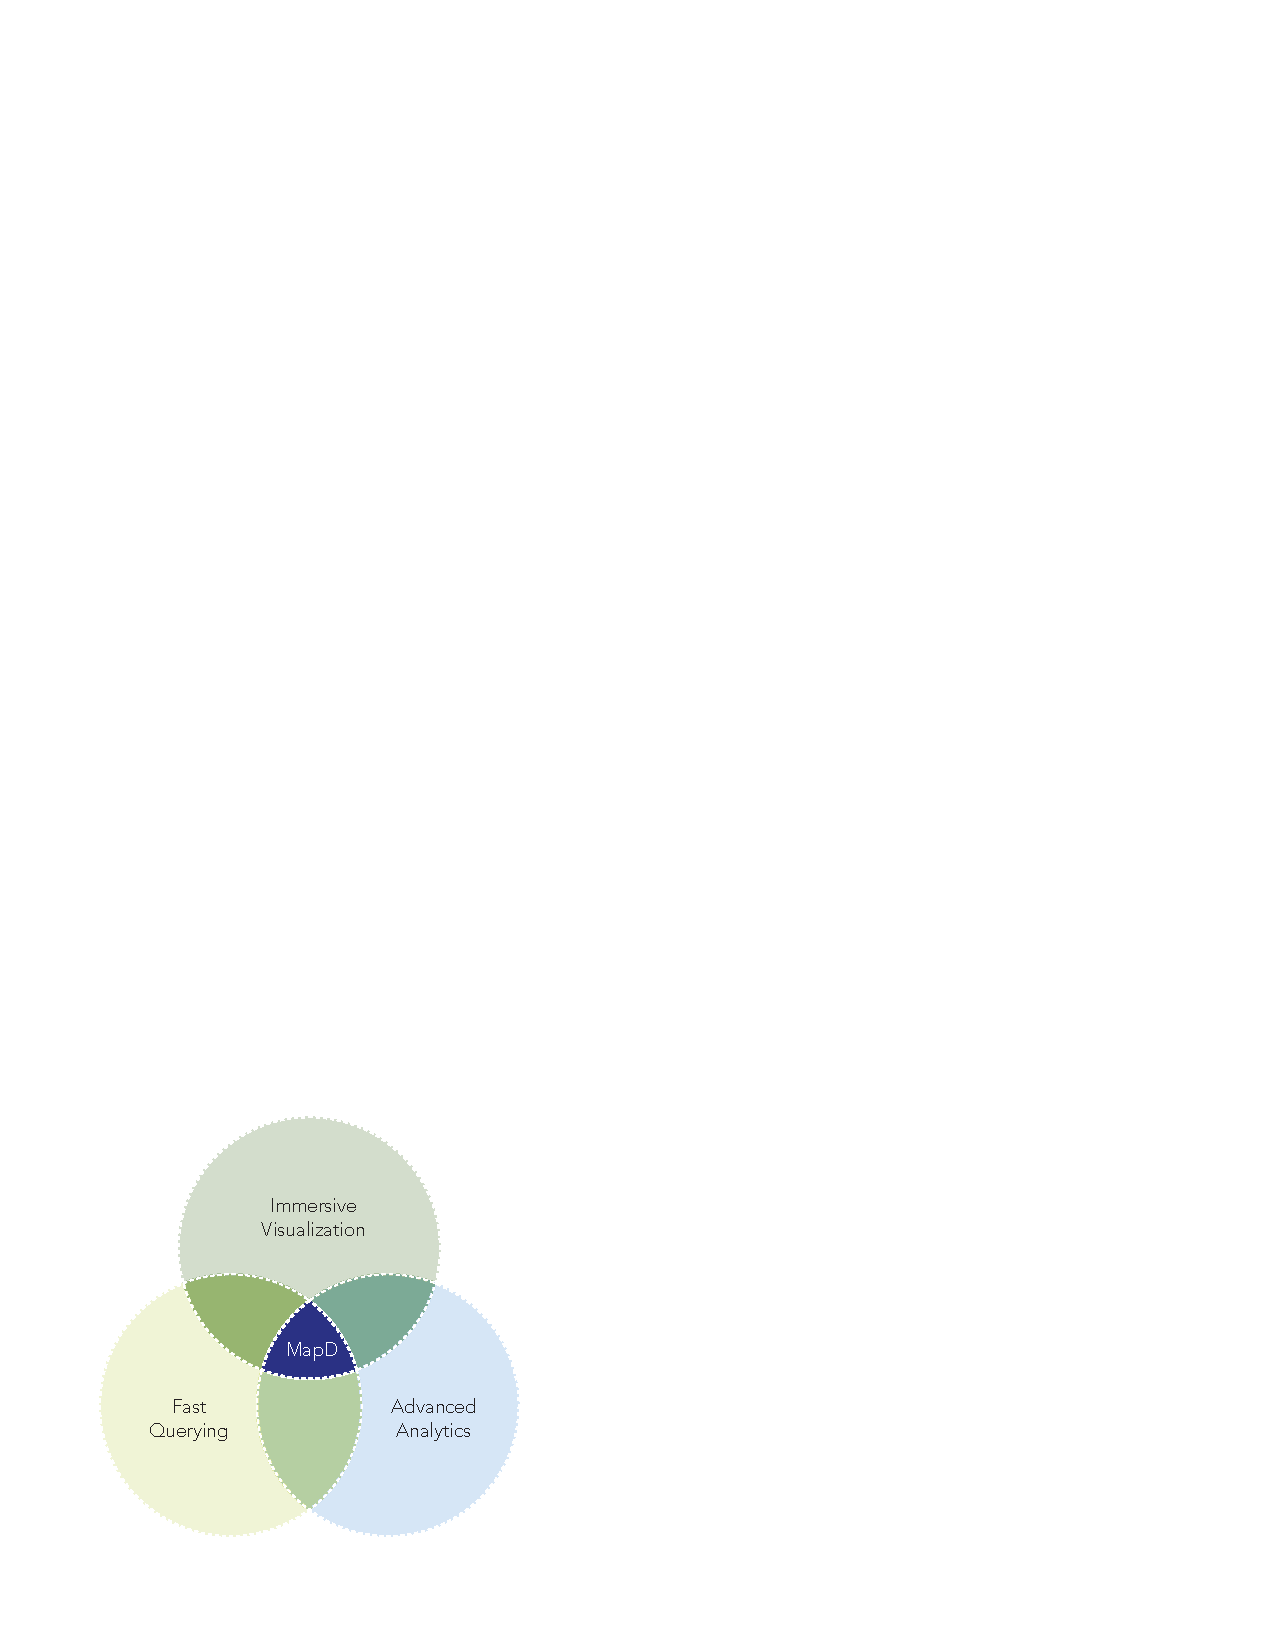
\includegraphics[width=0.38\textwidth]{mapd-diagram.pdf}
        \caption{MapD vision}
        \label{fig:mapd-diagram}
\end{figure}

\noindent
\textit{Processing Model:} 
MapD processes queries by compiling a query to executable code for the CPU and GPU.

\noindent
\textit{Query Placement \& Optimization:} 
The optimizer tries to split a query plan in parts, and processes each part on the most suitable processing device (e.g., text search using an index on the CPU and table scans on the GPU). MapD does not assume that an input data set fits in GPU RAM, and it applies a streaming mechanism for data processing.

\noindent
\textit{Transactions:} Not supported.

\noindent
\textbf{Performance:} While GPU performance and memory capacity are still rapidly increasing, in the current generation, up to eight GPU cards with 192GB total GPU memory can be installed in a single server, allowing data to be queried at rates approaching three terabytes per second by almost 40,000 cores. Furthermore, using the sophisticated graphics pipeline on each GPU, the data can be visualized in situ and sent to the client without the need for costly transfers to other platforms.

Although MapD was designed to deliver weightless data exploration straight to the browser, it is equally capable of processing programmatic SQL queries with blistering speed (at a rate over a trillion rows per second per server for certain workloads).

\begin{figure}[htb]
        \centering
        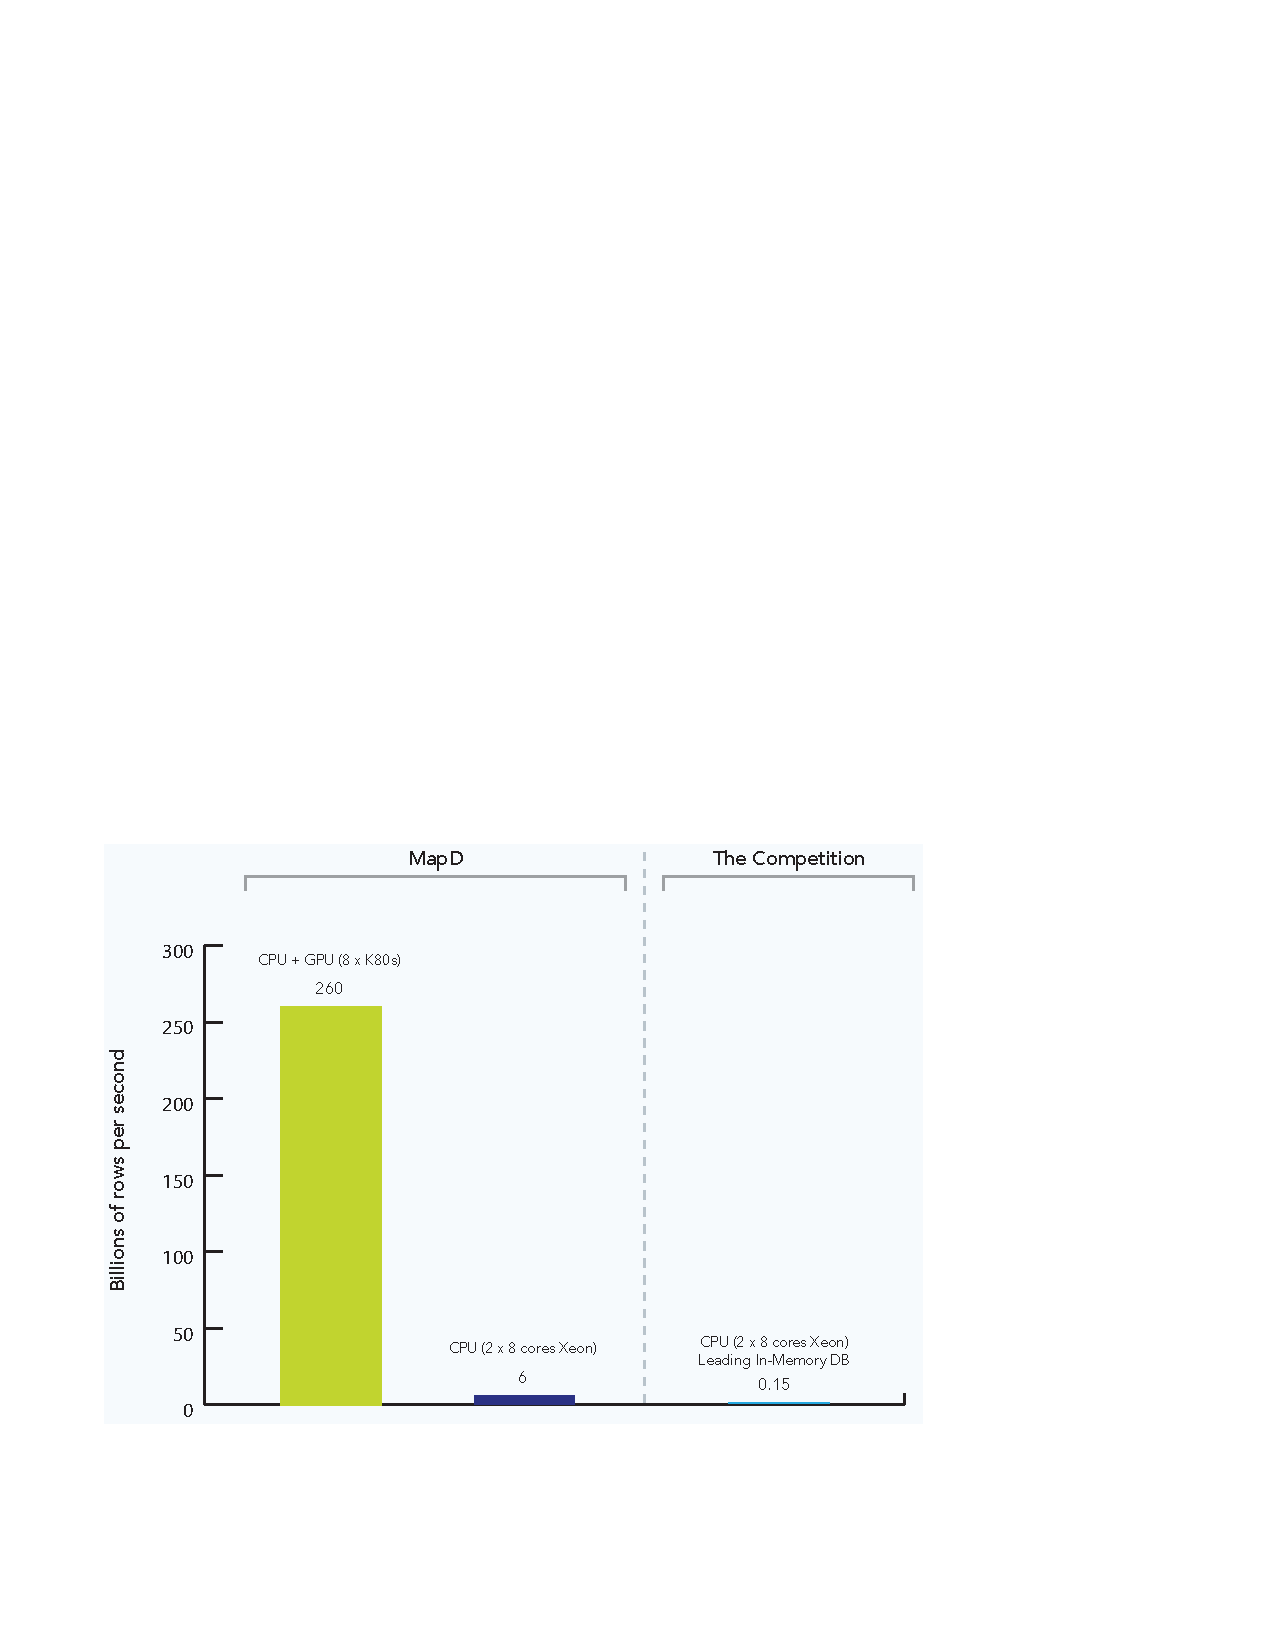
\includegraphics[width=0.48\textwidth]{mapd-graph.pdf}
        \caption{Map performance compared to leading in-memory database on 2-socket, 8-GPU system.}
        \label{fig:mapd-graph}
\end{figure}

\noindent
\textbf{The MapD platform uniquely:}
Caches the hot data in GPU memory such that no time is lost moving the data across the PCIe bus onto the GPU when a query is executed.

\bi
\ii \textit{Vectorizes execution} of queries whenever possible. Vectorized code allows the compute resources of a processor to process multiple data items simultaneously. This is a must to achieve good performance on GPUs, which can comprise thousands of execution units. Additionally, optimizing vectorized execution also translates well to CPUs, which increasingly have “\textit{wide}” execution units capable of processing multiple data items at once.
\ii Employs \textit{highly-optimized kernels} for common database operations. Although GPUs are extremely fast, GPU code often requires more optimization work than comparable CPU code to achieve the best performance. MapD is
the product of thousands of hours of benchmarking and testing to extract the maximum vectorized performance from both GPU and CPU.
\ii Compiles queries \textit{on the fly} for maximum execution speed.
\ii Executes queries \textit{simultaneously} on both CPU and GPU, or entirely on CPU if the working dataset cannot fit in GPU memory.
\ii Visualizes and performs complicated analytics on data in situ. Since the relevant data is already cached on the GPUs, MapD does not need to copy the query result set before rendering it (using the GPUs) or using it as input to a follow-on machine learning algorithm.
\ei

\subsection{Ocelot}
Heimel and others develop Ocelot\footnote{Source code available at: \href{http://goo.gl/GHeUv}{http://goo.gl/GHeUv}.}, which is an OpenCL extension of MonetDB, enabling operator execution on any OpenCL capable device, including CPUs and GPUs \cite{Heimel:2013}(Fig. \ref{fig:ocelot}).
\begin{figure}[htb]
        \centering
        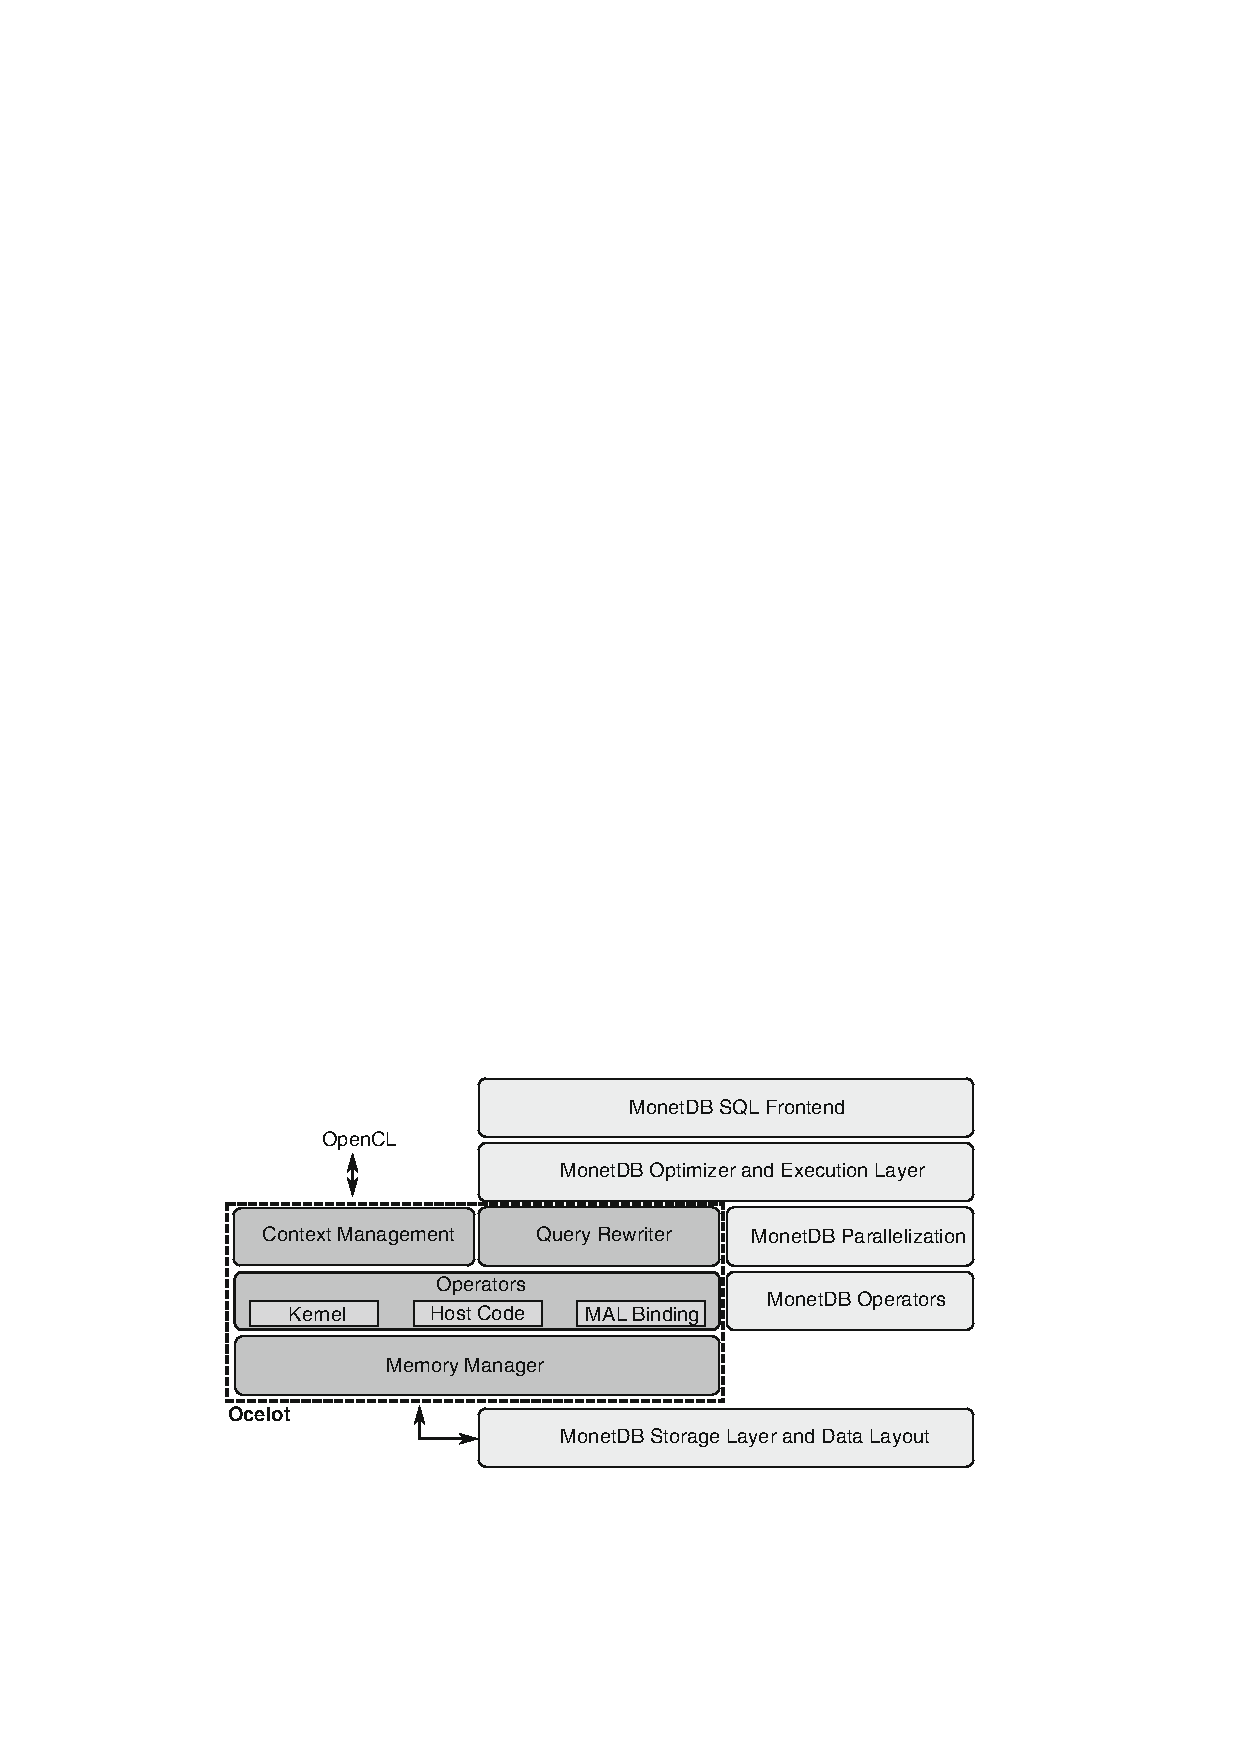
\includegraphics[width=0.48\textwidth]{ocelot.pdf}
        \caption{The architecture of Ocelot}
        \label{fig:ocelot}
\end{figure}

\noindent
\textit{Storage System:} 
Ocelot’s storage system is built on top of the \textit{in-memory} model of MonetDB. Input data is automatically transferred from MonetDB to the GPU when needed by an operator. In order to avoid expensive transfers, operator results are typically kept on the GPU. They are only returned at the end of a query, or if the device memory is too filled to fulfill requests. Additionally, Ocelot implements a \textit{device cache} to keep relevant input data available on the GPU.

\noindent
\textit{Storage Model:} 
Ocelot/MonetDB stores data column-wise in \textit{Binary Association Tables} (BATs). Each BAT consists of two columns: One (optional) head storing object identifiers, and one (mandatory) tail storing the actual values.

\noindent
\textit{Processing Model:} Ocelot inherits the \textit{operator-at-a-time} bulk processing model of MonetDB, but extends it by introducing \textit{lazy evaluation} and making heavy use of the OpenCL event model to forward operator dependency information to the GPU. This allows the OpenCL driver to automatically interleave and reorder operations, e.g., to hide transfer latencies by overlapping the transfer with the execution of a previous operator.

\noindent
\textit{Query Placement \& Optimization:} 
In MonetDB, each query plan is represented in the \textit{MonetDB Assembly Language} (MAL). Ocelot reuses this infrastructures and adds a new query optimizer, which rewrites MAL plans by replacing data processing MAL instructions of vanilla MonetDB with the highly parallel OpenCL MAL instructions of Ocelot.
Ocelot does not support cross-device process- ing, meaning it executes the complete workload either on the CPU or on the GPU.

\noindent
\textit{Transactions:} Not supported.

\subsection{OmniDB}
Zhang and others developed OmniDB\footnote{Source code available at: \href{https://code.google.com/p/omnidb-paralleldbonapu/}{https://code.google.com/p/omnidb-paralleldbonapu/}.}, a GDBMS aiming for good code maintainability while exploiting all hardware resources for query processing \cite{Zhang:2013}. 
The basic idea is to create a hardware oblivious database kernel (qkernel), which accesses the hardware via \textit{adaptors}. Each adapter implements a common set of operators decoupling the hardware from the database kernel (Fig. 8).
\begin{figure}[htb]
        \centering
        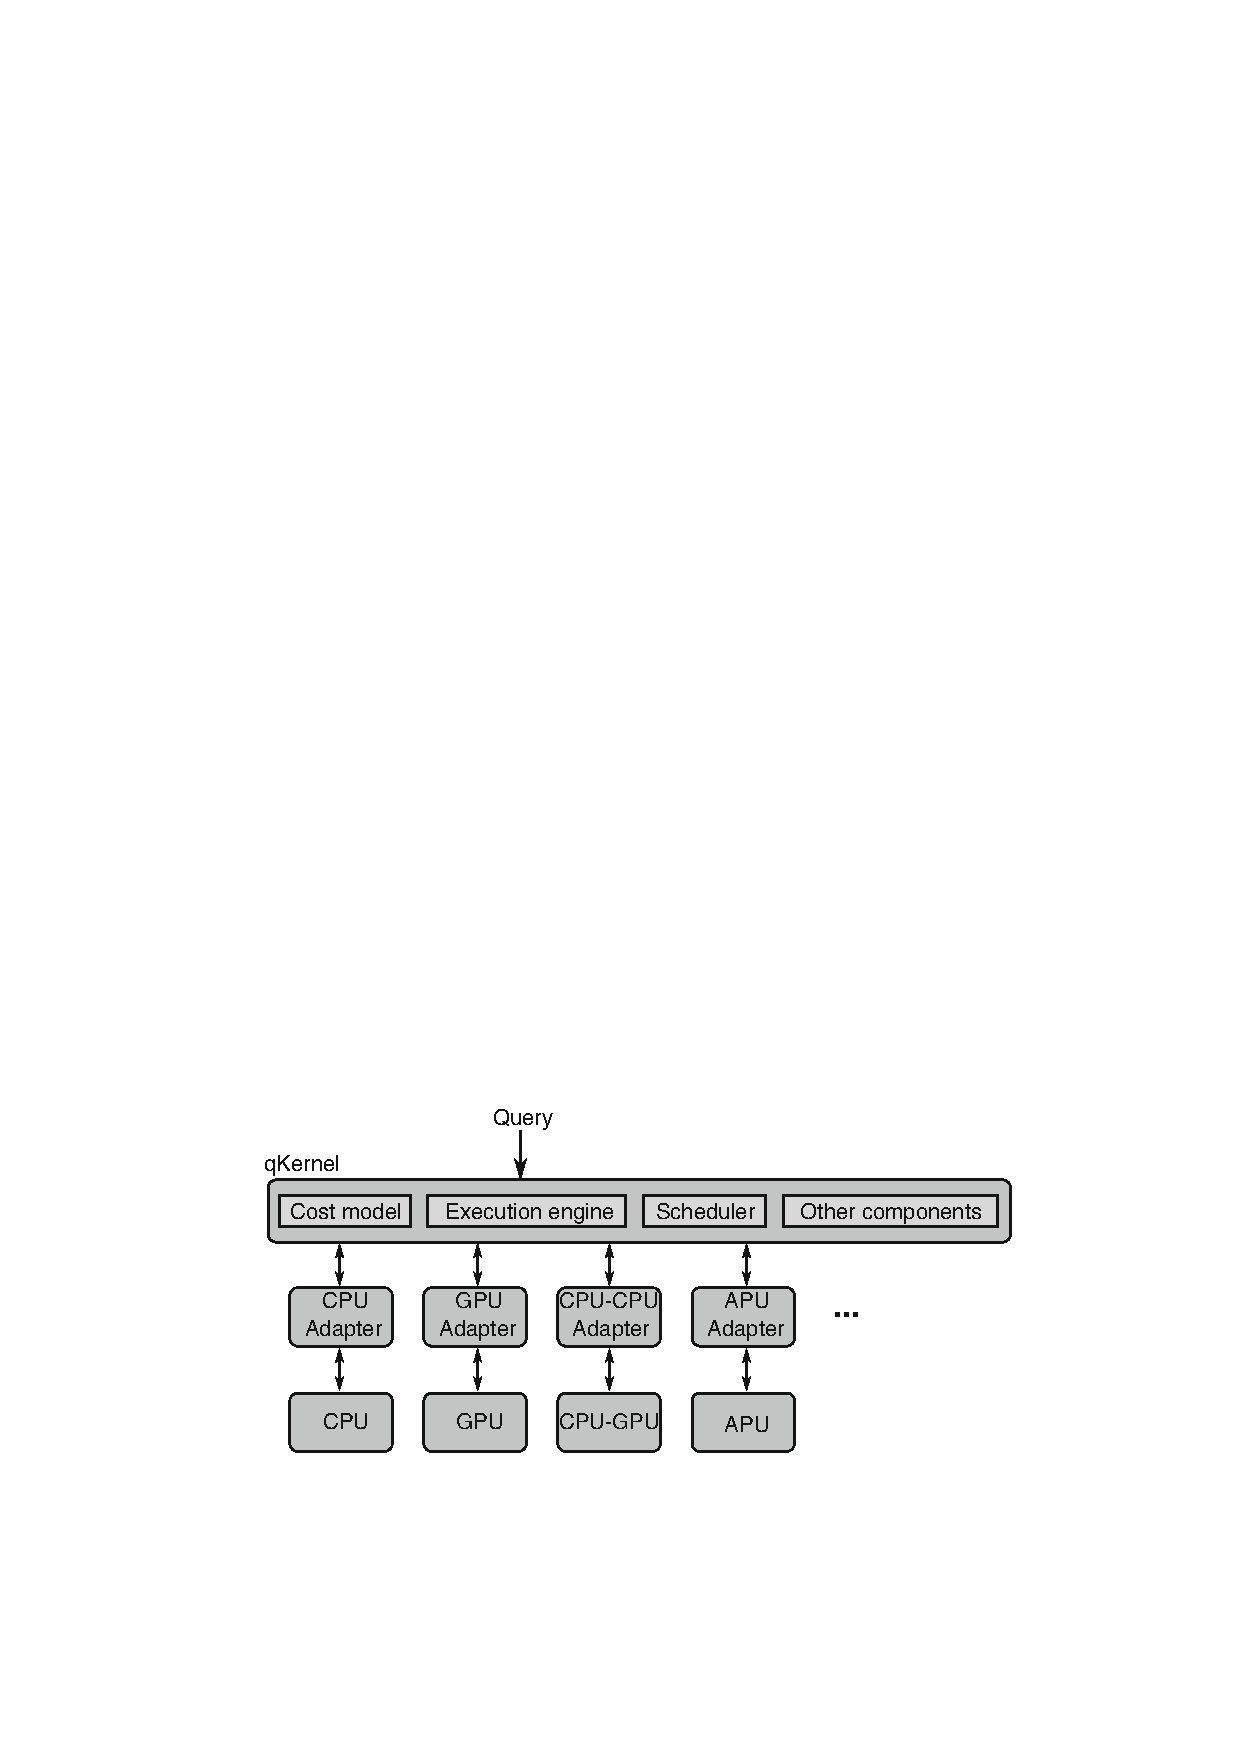
\includegraphics[width=0.48\textwidth]{omnidb.pdf}
        \caption{OmniDB: Kernel adapter design}
        \label{fig:omnidb}
\end{figure}

\noindent
\textit{Storage System \& Model:} 
OmniDB is based on GPUQP, and hence, has similar architectural properties to GPUQP. 
OmniDB keeps data in-memory in a column- oriented data layout.

\noindent
\textit{Processing Model:} 
OmniDB schedules and processes work units, which can vary in granularity (e.g., a work unit can be a query, an operator, or a chunk of tuples). Although it is not explicitly mentioned in the paper, the fact that OmniDB can process also chunks of tuples is a strong indicator that it supports block-oriented processing.

\noindent
\textit{Query Placement \& Optimization:} 
Regarding query placement and optimization, OmniDB chooses the processing device with highest throughput for a work unit. To avoid overloading a single device, OmniDB’s scheduler ensures that the workload on one processing device may not exceed a certain percentage of the average workload on all processing devices. The cost model relies on the adapters to provide cost functions for the underlying processing devices.

\noindent
\textit{Transactions:} Not supported.

\subsection{Virginian}
Bakkum and others develop Virginian\footnote{Source code available at: \href{https://github.com/bakks/virginian}{https://github.com/bakks/virginian}.}, which is a GPU-accelerated DBMS keeping data in main memory and supporting filter and aggregation operations on all processing devices \cite{Bakkum:2012}.

\noindent
\textit{Storage System:} 
Virginian uses no traditional caching of operators, but \textit{uniform virtual addressing} (UVA). This technique allows a GPU kernel to directly access data stored in pinned host memory. The accessed data is transferred over the bus transparently to the device and efficiently overlaps computation and data transfers.

\noindent
\textit{Storage Model:} 
Virgnian implements a data structure called \textit{tablet}, which stores fixed size values column oriented. Additionally, tables can handle variable sized data types such as strings, which are stored in a dedicated section inside the tablet. Thus, Virginian supports strings on the GPU. This is a major difference to other GDBMSs, which apply dictionary compression on strings first and work only on compressed values in the GPU RAM.

\noindent
\textit{Processing Model:} Virginian uses operator-at-a-time processing as basic query- processing model. It implements an alternative processing scheme. While most systems call a sequence of highly parallel primitives requiring one new kernel invocation per primitive, Virginian uses the opcode model, which combines all primitives in a single kernel. This avoids writing data back to global memory and reading it again in the next kernel ultimately resulting in block-wise processing on the GPU.

\noindent
\textit{Query Placement \& Optimization:} Virginian can either process queries on the CPU or on the GPU. Thus, there is no mechanism splitting up the workload between CPU and GPU processing devices and hence, no hybrid query optimizer is available.

\noindent
\textit{Transactions:} Not supported.

\section{Potential Optimizations}
We will now discuss and summarize potential optimizations, which a GDBMS may implement to make full use of the underlying hardware in a hybrid CPU/GPU system. 
Additionally, we briefly discuss existing approaches for each optimization. 
As already discussed, data transfers have the highest impact on GDBMS performance. 
Hence, every optimization avoiding or minimizing the impact of data transfers are mandatory. 
We refer to these optimizations as cross-device optimizations. 
Based on our surveyed systems, we could identify the following \textit{cross-device optimizations} :

\noindent
\textbf{Efficient Data Placement Strategy:} 
There are two possibilities to manage the GPU RAM. The first possibility is an explicit management of data on GPUs using a buffer-management algorithm. The second possibility is using mechanisms such as Unified Virtual Addressing (UVA), which enables a GPU kernel to directly access the main memory. 
Kaldewey and others observed a significant performance gain (3-8x) using UVA for Hash Joins on the GPU compared to the CPU \cite{Kaldewey:2012}. Furthermore, data has not to be kept consistent between CPU and GPU, because there is no “real” copy in the GPU RAM. However, this advantage can also be a disadvantage, because caching data in the GPU RAM can avoid the data transfer from the CPU to the GPU.

\noindent
\textbf{GPU-aware Query Optimizer:} 
A GDBMS should make use of all processing devices to maximize performance. Therefore, it should offload operations to the GPU. However, offloading single operations of a query plan does not necessarily accelerate performance. 
Hence, a GPU-aware optimizer has to identify sub plans of a query plan, which it can process on the CPU or the GPU \cite{He:2009}. Furthermore, the resulting plan should minimize the number of copy operations. 
Since optimizers are typically cost based, a GDBMS needs for each GPU operator a cost model. The most common approach is to use analytical models.
However, with the increasing hardware complexity, machine-learning-based models become increasingly popular.

\noindent
\textbf{Data Compression:}
The data placement and query optimization techniques attempt to avoid data transfers as much as possible. To reduce overhead in case a GDBMS has to perform data transfers, the data volume can be reduced by compression techniques. 
Thus, compression can significantly decrease processing costs \cite{Yuan:2013}. 

\noindent
\textbf{Overlap of Data Transfer and Processing:} 
The second way to accelerate processing, in case a data transfer needs to performed, is overlapping the execution of a GPU operator with a data transfer operation \cite{Yuan:2013}. This optimization keeps all hardware components busy, and basically narrows down the performance of the system to the PCIe bus bandwidth.

\noindent
\textbf{Pinned Host Memory:} 
The third way to accelerate query processing in case we have to perform a copy operation is keeping data in pinned host memory. This optimization saves one indirection, because the DMA controller can transmit data directly to the device \cite{Yuan:2013}. Otherwise, data has to be copied in pinned memory first, introducing additional latency in data transmission. However, using pinned host memory has the drawback that the amount of available pinned host memory is much smaller than the amount of unpinned memory (i.e., memory that can be paged to disk by the virtual memory manager). Therefore, a GDBMS has to decide which data it should keep in pinned host memory. It is still an open issue how much memory should be spent on a pinned host memory buffer for faster data transfers to the GPU.
Figure \ref{fig:cross-device-tree} illustrates the identified cross-device optimizations and the relationships between them.

\begin{figure}[htb]
        \centering
        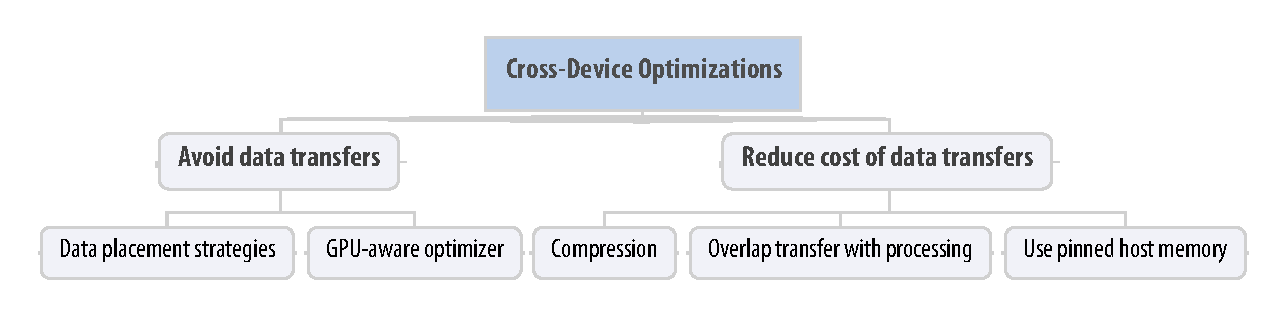
\includegraphics[width=0.5\textwidth]{cross-device-tree.pdf}
        \caption{Cross-device Optimizations}
        \label{fig:cross-device-tree}
\end{figure}

The second class of optimizations we identified, targets the efficiency of opera- tor execution on a single processing device. We refer to this class of optimizations as \textit{device-dependent optimizations}. 
Since we focus on GPU-aware systems, we only discuss optimizations for GPUs. 
Based on the surveyed systems, we summarize the following GPU-dependent optimizations:
\begin{figure}[htb]
        \centering
        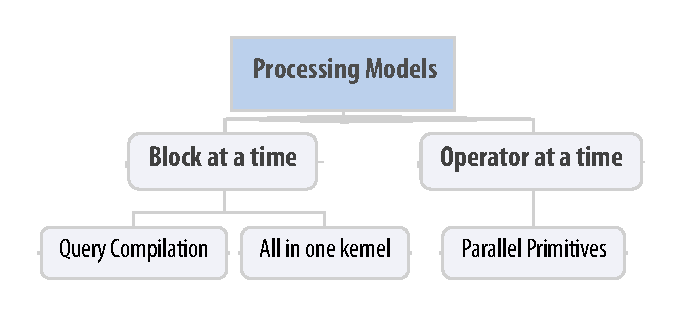
\includegraphics[width=0.45\textwidth]{device-dependent-tree.pdf}
        \caption{Device-dependent optimizations: Efficient processing models}
        \label{fig:device-dependent-tree}
\end{figure}
Figure \ref{fig:device-dependent-tree} illustrates the identified device-dependent optimizations and the relationships between them.

\noindent
\textbf{Block-oriented Query Processing:} 
A GDBMS can avoid the overhead of writing results of an operator back to a processing device’s main memory by processing data on a \textit{per block basis} rather than on a per operator basis. 
The idea is to process data already stored in the cache (CPU) or shared memory (GPU), which saves memory bandwidth and significantly increases performance of query processing \cite{Yuan:2013}. 
Additionally, \textit{block-oriented processing} is a necessary prerequisite for overlapping processing and data transfer for single operations and allows for a more fine grained workload distribution on available processing devices \cite{Zhang:2013}. 
Note that traditional pipelining of blocks between GPU operators is not possible, because inter-kernel communication is undefined. 
While launching a new kernel for each block is likely to be expensive, \textit{query compilation} and \textit{kernel fusion} are promising ways to allow block-oriented processing on the GPU as well.

\noindent
\textbf{Compilation-based Query Processing:} 
Compiling queries to executable code is a common optimization in main-memory DBMSs. 
As already discussed, query compilation allows for block-oriented processing on GPUs as well and achieves a significant speedup compared to primitive-based query processing (e.g., operator-at-a-time processing \cite{He:2009}). 
However, query compilation introduces additional overhead, because compiling a query to executable code typically is more expensive than building a physical query execution plan. Yuan and others overcome this shortcoming by pre-compiling operators. Thus, they only need to compile the query plan itself to a driver program \cite{Yuan:2013}. 
A similar approach called \textit{kernel weaver} is used by Wu and others \cite{Wu:2012}. 
They combine CUDA kernels for relational primitives into one kernel. This has the advantage that the optimization scope is larger and the compiler can perform more optimizations. However, the disadvantage is the increased compilation time. Rauhe and others introduce in their approach two processing phases: \textit{compute} and \textit{accumulate}. In the compute phase, a number of threads are assigned to a partition of the input data and each thread performs all operations of a query on one tuple and then, continues with the next tuple, until the thread processed its partition. 
In the accumulate phase, the intermediate results are combined to the final result \cite{Rauhe:2013}.

\noindent
\textbf{All-in-one Kernel:} 
A promising alternative to compilation-based approaches is to combine all relational primitives in one kernel \cite{Bakkum:2012}. Thus, a relational query has to be translated to a sequence of op codes. An op code identifies the next primitive to be executed. Therefore, it is basically an on-GPU virtual machine, which saves the initial overhead of query compilation. However, the drawback is a limited optimization scope compared to \textit{kernel weaver}  \cite{Wu:2012}.

\noindent
\textbf{Portability:} 
Until now, we mainly discussed performance optimizations. How- ever, each of the discussed optimizations are mainly implemented device dependent. This increases the overall complexity of a GDBMS. The problem gets even more complex with new processing device types such as accelerated processing units or the Intel Xeon Phi. Heimel and others implemented a hardware oblivious DBMS kernel in OpenCL and still achieved a significant acceleration of query processing \cite{Heimel:2013}. 
Zhang and others implemented \textit{q-kernel}, a hardware-oblivious database kernel using device adapters to the underlying processing devices \cite{Zhang:2013}. It is still not clear which part of a kernel should be hardware oblivious and which part should be hardware aware. 
For the parts that have to be hardware aware, modern software engineering methods such as software product lines can be used to manage the GDBMS’s complexity \cite{Broneske:2014}.

\section{Reference Architecture for GDBMSs}
Based on our in-depth survey of existing GDBMSs, we now derive a reference architecture for GDBMSs. After careful consideration of all surveyed systems, we decided to use the GPUQP/OmniDB \cite{Zhang:2013} architecture as basis for our reference architecture, because they already include a major part of the common properties of the surveyed systems. We illustrate the reference architecture in Fig. \ref{fig:gdbms}.
\begin{figure}[htb]
        \centering
        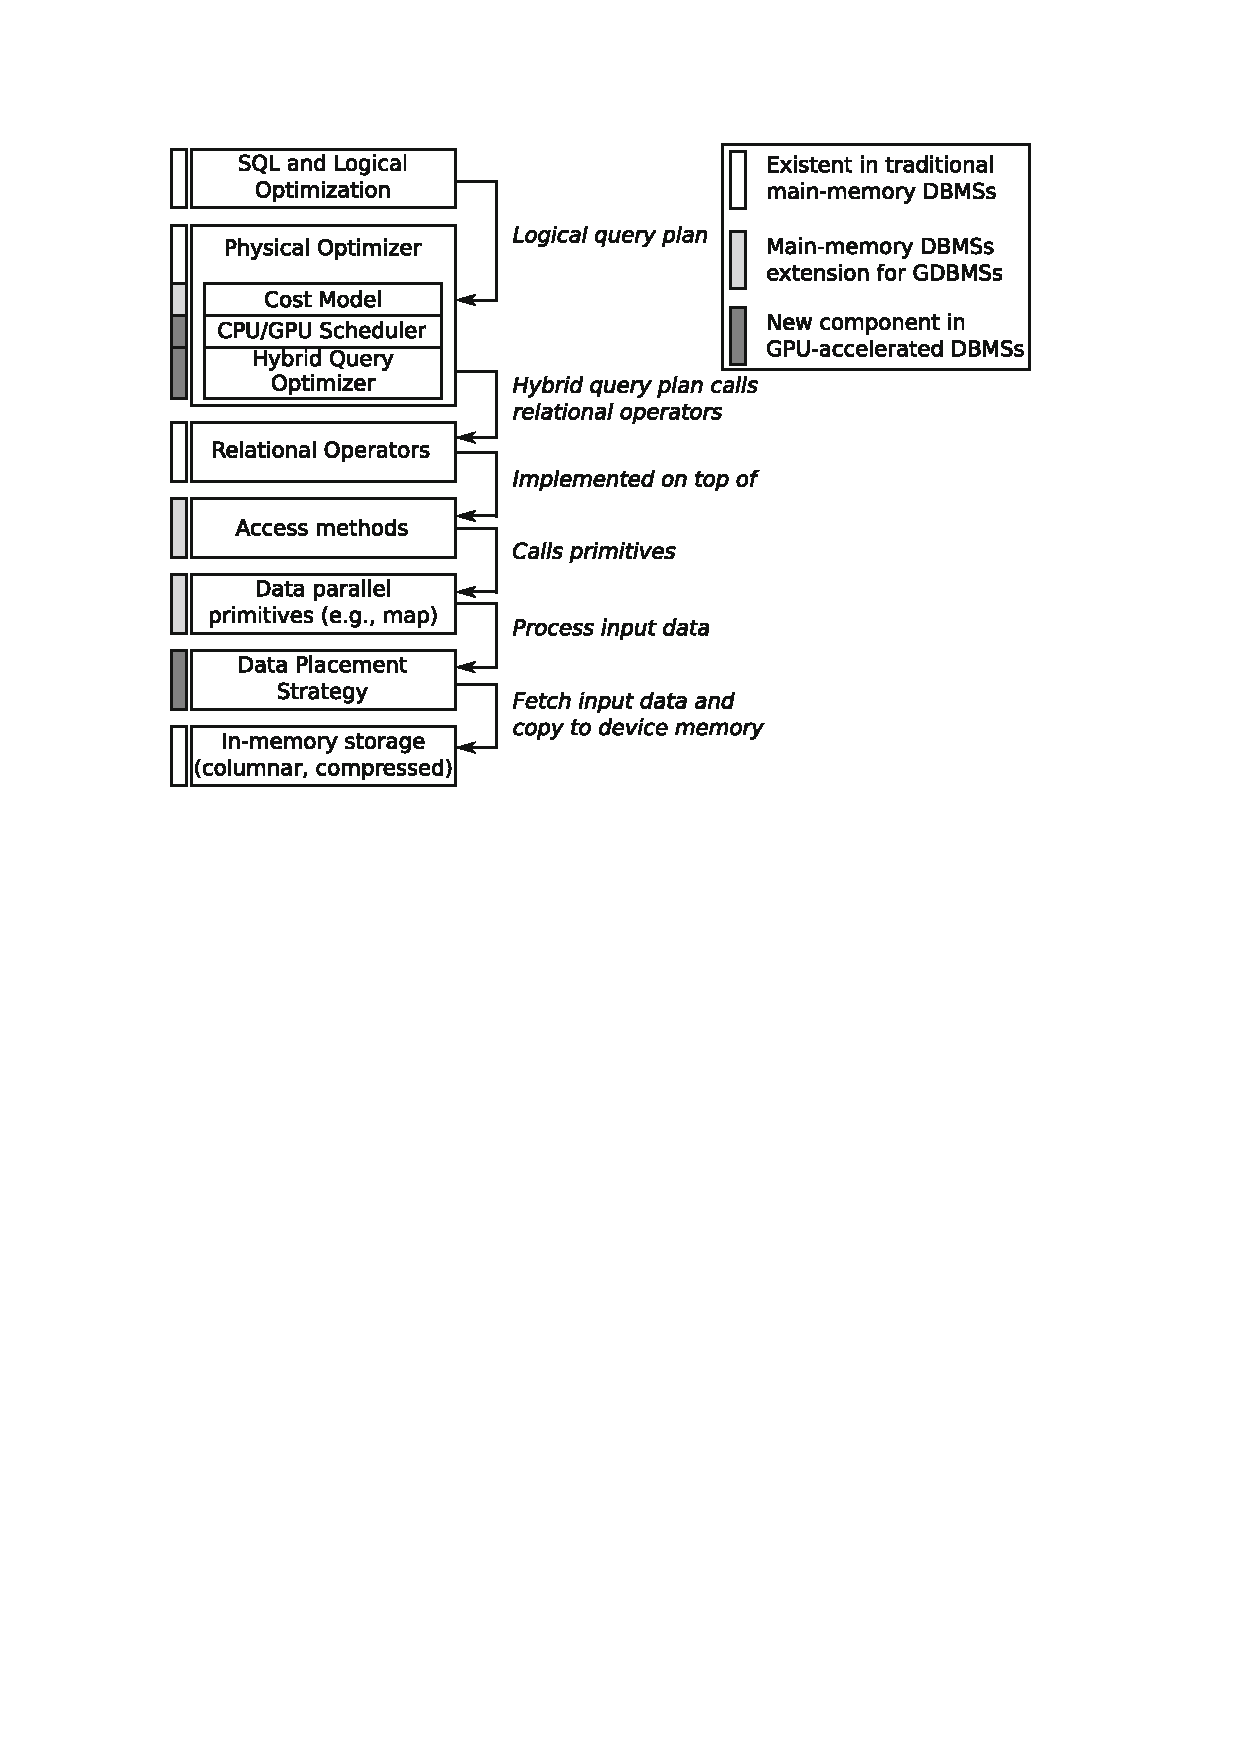
\includegraphics[width=0.48\textwidth]{gdbms.pdf}
        \caption{Layered architecture of GDBMSs}
        \label{fig:gdbms}
\end{figure}

We will describe the query-evaluation process in a top-down view. On the upper levels of the query stack, a GPU-accelerated DMBS is virtually identical to a “traditional” DBMS. It includes functionality for integrity control, parsing SQL queries, and performing logical optimizations on queries. Major differences between main-memory DBMSs and GDBMSs emerge in the physical optimizer. While classical systems choose the most suitable access structure and algorithm to operate on the access structure, a GPU-accelerated DBMS has to additionally decide for each operator on a processing device. For this task, a GDBMS needs refined13 cost models that also predict the cost for GPU and CPU operations. Based on these estimates, a scheduler can allocate the cheapest processing device. Furthermore, a query should make use of multiple processing devices to speed up execution. Hence, the physical optimizer has to optimize hybrid CPU/GPU query plans, which significantly increases the optimization space.

Relational operations are implemented in the next layer. These operators typically use access structures to process data. In GDBMSs, access structures have to be reimplemented on GPUs to achieve a high efficiency. However, depending
on the processing device chosen by the CPU/GPU scheduler, different access structures are available. This is an additional dependency the query optimizer needs to take into account.

Then, a set of parallel primitives can be applied to an access structure to process a query. In this component, the massive parallelism of CPUs and GPUs is fully used to speed up query processing. However, a GPU operator can only work on data stored in GPU memory. Hence, all access structures are built on top of a data-placement component, that caches data on a certain processing device, depending on the access patterns of the workload (e.g., certain columns for column scans or certain nodes of tree indexes). Note that the data- placement strategy is the most performance critical component in a GDBMS due to the major performance impact of data transfers.

The backbone of a GDBMS is a typical in-memory storage, which frequently stores data in a column-oriented format. Compression techniques are not only beneficial in keeping the major part of a database in-memory, compression also reduces the impact of the PCIe bottleneck.

\subsection{Extension Points for MMDBMSs}
In summary, we can extend most \textit{main-memory DBMSs} (MMDBMSs) supporting column- oriented data layout and bulk processing to be GPU-accelerated DBMSs. 
We identify the following extension points: Cost models, CPU/GPU scheduler, hybrid query optimizer, access structures and algorithms for the GPU, and a data placement strategy.

\noindent
\textbf{Cost Models:} For each processor, we need to estimate the execution time of an operator. This can be either done by \textit{analytical} cost models or \textit{learning-based} approaches.

\noindent
\textbf{CPU/GPU Scheduler:} Based on the cost models, a scheduler needs to allocate processing devices for a set of operators.

\noindent
\textbf{Hybrid Query Optimizer:} The query optimizer needs to consider the data transfer bottleneck and memory requirements of operators to create a suit- able physical execution plan. Thus, the optimizer should make use of cost models, a CPU/GPU scheduler, and heuristics minimizing the time penalty of data transfers.

\noindent
\textbf{Access structures and algorithms for the GPU:} In order to support GPU- acceleration, a DBMS needs to implement access structures on the GPU (e.g., columns or B+-trees) and operators that work on them. 

\noindent
\textbf{Data Placement Strategy:} A DBMS needs to keep track of which data is stored on the GPU, and which access structure needs to be transferred to GPU memory. Aside from a manual memory management, it is also possible to use techniques such as UVA and let the GPU driver handle the data transfers transparently to the DBMS. However, this may result in less efficiency because a manual memory management can exploit knowledge about the DBMS and the workload.

Implementing these extensions is a necessary precondition for a DBMS to sup- port GPU co-processing efficiently.



\section{Conclusion}
The pioneer of modern co-processors is the GPU, and many prototypes of GPU-accelerated DBMSs have emerged over the past seven years implementing new co-processing approaches and proposing new system architectures. We argue that we need to take into account tomorrows hardware in today's design decisions. Therefore, in this paper, we theoretically explored the design space of GPU-aware database systems. 

In summary, we argue that a GDBMS should be an \textit{in-memory}, \textit{column-oriented} DBMS using the \textit{block-at-a-time} processing model, possibly extended by a \textit{just-in-time-compilation} component. The system should have a query optimizer that is aware of \textit{co-processors} and \textit{data-locality}, and is able to distribute a workload across all available (co-)processors.


\bibliographystyle{abbrv}
\bibliography{sqlonhadoop}

\end{document}
